\documentclass[12pt,oneside,openany]{report}
% Márgenes APA 2.54 cm
\usepackage[a4paper,margin=2.54cm]{geometry}
\usepackage[T1]{fontenc} % mejor codificación de fuentes para español
\usepackage[spanish]{babel}
\usepackage[utf8]{inputenc}
\usepackage{csquotes}
\usepackage{amsmath}
\usepackage{listings}
\lstset{breaklines=true}

\pagestyle{plain}

\usepackage{graphicx}
\graphicspath{{./images/}}
\usepackage{caption}
\usepackage{array}

\usepackage{tocbibind}

\usepackage[normalem]{ulem}
\usepackage{xcolor}
\definecolor{edit30sept}{HTML}{e3256b}

\usepackage{hyperref}
\hypersetup{
    colorlinks=true,
    linkcolor=black,
    filecolor=magenta,      
    urlcolor=black,
    citecolor=black,
}
\urlstyle{same}

\usepackage{microtype}
\usepackage{lmodern} % fuentes vectoriales para evitar error microtype con tamaños sustituidos

% Interlineado APA
\usepackage{setspace}

% Sangría estándar APA 0.5 pulgadas ~ 1.27 cm
\setlength{\parindent}{1.27cm}

% Estilo de referencias APA
\usepackage[backend=biber,style=apa,sorting=nyt,language=spanish]{biblatex}
\DeclareLanguageMapping{spanish}{spanish-apa}
% Improved workaround for datecircaprint
\AtBeginDocument{%
  \providecommand{\datecircaprint}{%
    \ifcsdef{bibstring}{\bibstring{circa}}{\textit{circa}}%
    \ifcsdef{printdelim}{\printdelim{datecircadelim}}{}%
  }%
}
\addbibresource{references/bibliography.bib}
\addbibresource{references/videography.bib}

% Para regenerar Tabla de contenidos tras un error: `make clean` y luego `make main` (2-3 pasadas automáticas)

% Nota: Para citas con Biblatex apa, usar \parencite y \textcite.

\let\cleardoublepage=\clearpage

\AtBeginEnvironment{quote}{\small}
% Captions en mismo tamaño y doble espacio (controlado por setspace)
\captionsetup{font=normalsize}

% Nombres de listas acorde normativa en español
\renewcommand{\listfigurename}{Lista de Figuras}
\renewcommand{\listtablename}{Lista de Tablas}

\begin{document}

% Interlineado doble global
\doublespacing

\thispagestyle{empty}
\begin{titlepage}
\renewcommand*{\thepage}{Title}

    \begin{center} 
        \vspace*{3cm}
        
        {\fontsize{16pt}{22pt}\selectfont\textbf
            {Significación social y supervivencia simbólica en la producción de imagen artística sobre la resistencia y crisis del Hospital San Juan de Dios, Bogotá, 2000-2015}
        }


        
        \vspace{1.5cm}
        
        \text{Por:}
        
        \vspace{0.5cm}
        
        	JUAN CARLOS ARROYO SOSA, B.A. \\

        \vspace{1.5cm}
        
        	Tesis presentada a la Facultad de Artes y Humanidades \\
            de la Universidad de Caldas, en cumplimiento parcial de los requisitos \\
            para el grado de Magister en Diseño y Creación Interactiva

        
        \vspace{2.5cm}
        
        Asesora de Tesis:\\

        \vspace{0.5cm}
        
        BEATRIZ DEL CARMEN PERALTA DUQUE, Phd.\\
        
        \vspace{3cm}
        
            Universidad de Caldas\\
            \vspace{0.5cm}
            Artistic-2.0 license 2024. 
    
    \end{center}

\end{titlepage}
\cleardoublepage

\pagenumbering{roman}
\setcounter{page}{1}

\phantomsection
\addcontentsline{toc}{chapter}{Declaración de ética}
\section*{Declaración de ética}
\setlength{\parskip}{1em}

Yo, quién escribe este texto, he sido durante años un silencioso observador de el caso del San Juan, y como afectado contiguo al drama social derivado de la crisis y fin de los servicios hospitalarios, he visto los síntomas de decadencia funcional, deterioro de las edificaciones, y el drama humano vivido por las personas alrededor de la persistencia en las distintas formas de resistir al fin del HJSD. Una de esas trabajadoras a las que aún se les adeuda su liquidación, es mi madre, la enfermera Berenice Sosa o como aún después de tantos años de no ejercer su profesión, sus compañeras del San Juan le siguen diciendo “jefe Berenice”.

Esta investigación titulada \textit{Significación social y supervivencia simbólica en la producción de imagen artística sobre la resistencia y crisis del Hospital San Juan de Dios, Bogotá, 2000-2015} se ha realizado respetando los principios éticos fundamentales de integridad, transparencia y respeto hacia las personas y los materiales involucrados.  

La recolección de datos incluyó el uso de material de registro de obra artística, consulta bibliográfica, así como registro fotográfico personal y cedido temporalmente para consulta por ex trabajadores del hospital, quienes colaboraron de manera voluntaria y con su consentimiento informado. Se garantizó la confidencialidad de los participantes y el uso adecuado de los recursos proporcionados, asegurando que sus contribuciones fueran tratadas con el mayor respeto y se emplearan exclusivamente con fines académicos y de investigación.  

El estudio busca promover la comprensión de las dimensiones simbólicas y sociales de la resistencia y crisis del Hospital San Juan de Dios, contribuyendo a preservar su memoria histórica. Se evitó cualquier manipulación de la información recopilada y se actuó con responsabilidad frente a los derechos de los artistas, autores y participantes involucrados en este proceso.  

Esta tesis se adhiere a los principios éticos de la investigación académica y se compromete a actuar en beneficio de la verdad, el conocimiento y el reconocimiento cultural. 
\pagebreak

\phantomsection
\addcontentsline{toc}{chapter}{Resumen}
\section*{Resumen}
\setlength{\parskip}{1em}

Esta investigación aborda los desafíos de las trayectorias convertidas en imagen relacionadas con los derechos laborales del arquetipo de enfermera del Hospital San Juan de Dios (HSJD), enfocándose en la experiencia personal de mi madre durante la crisis del hospital como \textit{wicked problem}. La pregunta central que guía este estudio es: ¿Cómo la imagen artística sobre la crisis y resistencia del HSJD entre 2000 y 2015 contribuye a la significación y supervivencia simbólica de este evento en la memoria colectiva?.

De acuerdo con las referencias bibliográficas y audiovisuales consultadas, la belleza estética del hospital, el atractivo de la ruina y la complejidad histórica han generado múltiples perspectivas de creadores visuales, artistas, periodistas e investigadoras académicas que han observado y documentado el HSJD. \textcolor{edit30sept}{Sin embargo, esta prolífica producción no ha logrado generar para las enfermeras satisfacción en términos de justicia laboral y simbólica. La situación se presenta como un entramado complejo, lleno de expectativas fallidas, en el que al menos 3.640 personas quedaron desempleadas y aproximadamente 1.500 trabajadores no recibieron su liquidación.}

La investigación se desarrolla como una meta-composición estética y documental que trasciende la mera documentación o el análisis sociopolítico. Se sustenta en los campos de la antropología de la imagen, estudios visuales y sociosemióticos, para crear un fundamento argumentativo que permita «trabajar» con imágenes, que es, en esencia, pensar a través de las imágenes.

Metodológicamente, se operacionaliza el análisis mediante la apropiación de la idea de montaje, complementada con la identificación de imaginarios sociales y estructuras semióticas denominadas imágenes-síntoma y anacronismos. Esta aproximación permite interpretar cómo diversas acciones simbólicas, argumentales y estéticas evidencian una intensa producción visual en torno a la crisis del HSJD.

Los resultados revelan que los registros de estas acciones conforman un \textcolor{edit30sept}{ \emph{corpus}} de imágenes que permite interpretar tanto los síntomas visuales de la crisis sistémica como el deterioro arquitectónico y patrimonial en su interacción con el drama humano y social. La investigación demuestra cómo las representaciones visuales del HSJD trascienden la mera documentación para convertirse en evidencias del drama humano y la defensa de un bien público. \textcolor{edit30sept}{La tesis expone, mediante la metodología del montaje y la meta-composición estética y documental, la disrupción del fenómeno del San Juan, mostrando cómo estas operaciones visuales ofrecen oportunidades de reconfiguración de sentido en la memoria colectiva.}

Este estudio contribuye al campo del diseño y creación interactiva al proponer una metodología específica para el análisis de memoria social a través de la imagen, donde el montaje artístico se integra como medio de exploración y validación de hipótesis sobre la supervivencia simbólica de eventos críticos en el imaginario colectivo.

\vspace{1cm}
\textbf{Palabras clave:} \textcolor{edit30sept}{Meta-composición estética, montaje visual, imagen-síntoma, interfaz de memoria, crisis hospitalaria, Hospital San Juan de Dios Bogotá.}
\pagebreak


\phantomsection
\addcontentsline{toc}{chapter}{Dedicatoria}
\section*{Dedicatoria}

\vspace{2cm}

A todas las personas (vivas o muertas, locas o cuerdas) que han luchado por sus derechos laborales y el espíritu del cuidado humano en el Hospital San Juan de Dios de Bogotá.

\vspace{4cm}

\subsection*{Agradecimientos}
A mi esposa, quien me ha acompañado con amor y paciencia en este proceso; a mi madre, cuyo ejemplo de lucha y resistencia ha sido una inspiración constante; a mis profesores y tutores; y a todas las personas que, de una forma u otra, contribuyeron a la realización de este trabajo. Su apoyo ha sido un pilar fundamental a lo largo de este viaje, especialmente en los momentos en que las dificultades de la vida hicieron que observar y escribir se convirtieran en un refugio y una fuente de alivio.
\pagebreak

\phantomsection
\addcontentsline{toc}{chapter}{Licencia}
\section*{Artistic License 2.0}

El autor ha decidido licenciar esta obra bajo los términos de la Artistic License 2.0, permitiendo que cualquier persona:
\begin{itemize}
    \item Copie, modifique y distribuya el trabajo original o modificado.
    \item Cree versiones derivadas de la obra, siempre y cuando se indique claramente que se realizaron modificaciones.
\end{itemize}

\subsection*{Términos de la Licencia}

Al usar esta obra, aceptas que:

\begin{itemize}
    \item Debes incluir un aviso claro que indique si el trabajo ha sido modificado y qué cambios se han realizado.
    \item No puedes utilizar el nombre del autor original para promocionar productos derivados sin permiso explícito.
    \item El código fuente o el material base debe estar accesible para cualquier versión distribuida.
\end{itemize}

Para más información sobre la licencia, consulta el texto completo en inglés en el siguiente enlace: \href{https://opensource.org/licenses/Artistic-2.0}{Artistic License 2.0}.

---

\subsection*{Aclaración sobre fotografías y registros de obras}

Las imágenes de registro de obras de otros creadores y las fotografías incluidas en esta tesis, en particular aquellas compartidas por las extrabajadoras del Hospital San Juan de Dios (HSJD) y referidas en el texto, \underline{son de autoría y licencia de sus propios autores}.

Estas imágenes no comparten la licencia Artistic License 2.0 del texto de la tesis. Su uso y distribución están sujetos a los derechos de autor y licencias aplicables según lo determinado por sus respectivos autores.

Se recomienda contactar directamente a los autores o titulares de los derechos de las imágenes si se desea obtener más información sobre sus condiciones de uso.


\renewcommand{\contentsname}{Tabla de contenidos}
% Nota: compilar al menos 2 veces para regenerar TOC después de cambios.
\cleardoublepage
\phantomsection
\tableofcontents
\newpage

\pagenumbering{arabic}
\setcounter{page}{1}

\chapter{Conceptualización del problema}
\section*{Introducción al fenómeno}

La crisis del HSJD emerge como un laboratorio social donde el diseño y la creación interactiva pueden explorar las dinámicas de transformación institucional, memoria colectiva y resistencia ciudadana. Más allá de una indagación entre registros documentales o artísticos, este estudio pretende señalar cómo diversas acciones simbólicas, argumentales, documentales y estéticas evidencias de una intensa atracción visual en torno a la crisis del HSJD, los registros de estas acciones nos brindan un corpus de imágenes con potencial para interpretar los síntomas visuales de la crisis sistémica, así como los deterioros arquitectónicos y patrimonials en juego con el drama humano y social.

El caso del Hospital San Juan es emblemático dentro del contexto de las crisis sociales e institucionales generadas por los cambios masivos en los sistemas de salud orientados al servicio público. ¿Cómo comprender, explicar e interpretar los registros visuales y las obras que serán tratadas como \guillemotleft evidencias\guillemotright\ que articulan el drama humano y la defensa de un bien público?. 

A estas evidencias las denominamos imagen-síntoma, una presencia disruptiva en la imagen que interrumpe el curso normal de la representación: supervivencias, latencias y reapariciones que habitan las imágenes. La metodología aplicada a la colección visual de memoria social permite abordar el fenómeno a través de la imagen.

El concepto de imagen-síntoma\footnote{\begin{quote}La idea de la imagen como síntoma es lo que quiere tomar Didi-Huberman de Freud y aplicarlo al campo de la historia del arte. Por supuesto, no sobra decir que se trata de dos disciplinas muy distintas, que la experiencia de las imágenes oníricas no es igual a la de las imágenes artísticas. Aun así, el uso del carácter sintomático de la imagen en la historia del arte no es tan diferente al del análisis de los sueños. Sólo que aquí, en lugar de evocar lo onírico, Didi-Huberman lo utilizará para nombrar esa perturbación que lo visual causa dentro de lo visible. \parencite[p. 37]{VegaArevalo2017}\end{quote}} resulta fundamental para comprender cómo las representaciones visuales del HSJD trascienden la mera documentación para convertirse en manifestaciones de tensiones sociales más profundas. Según Didi-Huberman, estas imágenes actúan como síntomas que revelan conflictos latentes en el tejido social.

\begin{quote}
Si la imagen es un síntoma -en el sentido crítico y no clínico del término-, si la imagen es un malestar en la representación, es porque indica un futuro de la representación, un futuro que no sabemos aún leer, ni, incluso, describir. \parencite[p. 177]{DidiHuberman2011}
\end{quote}

Este estudio indaga en el papel fundamental de la imagen para la contemplación profunda de los fenómenos sociales, ofreciendo nuevas perspectivas para comprender su complejidad y contribuyendo al debate sobre el papel del arte y el diseño en los procesos de cambio social y la construcción de memoria colectiva.

El diseño, entendido como práctica crítica y performativa, permite desvelar las capas de significado ocultas en los registros visuales. No se trata solo de documentar, sino de construir narrativas que revelen las tensiones sociales subyacentes. Las imágenes del HSJD se convierten así en interfaces de memoria, donde cada fragmento, cada ruina, cada registro artístico funciona como un nodo de información compleja.

La creación interactiva se presenta como sugerencia para trascender la observación pasiva, invitando a una participación activa en la construcción de sentido. En este contexto, las obras artísticas y los registros visuales no son meros documentos, sino dispositivos de activación memorial que permiten:

\begin{itemize}
    \item Desarticular narrativas oficiales sobre el abandono institucional
    \item Visibilizar las experiencias de los trabajadores y comunidades afectadas
    \item Generar nuevas formas de comprensión y elaboración del conflicto social
\end{itemize}

\section*{Contextualización histórica}

El Hospital San Juan de Dios de Bogotá fue fundado en 1723 como un centro de atención médica y asistencia social para los más necesitados. A lo largo de los siglos, el hospital se convirtió en un referente de la salud pública en Colombia, atendiendo a miles de pacientes y formando a generaciones de profesionales de la salud. Sin embargo, a partir de la década de 1990, el HSJD comenzó a experimentar una serie de crisis institucionales y financieras que llevaron a su cierre.

En el año 2001, coincidiendo con la salida del último paciente, “3.640 personas quedaron desempleadas, y aproximadamente 1.500 trabajadores no recibieron la liquidación correspondiente por sus años de servicio” \parencite{Castiblanco2017}. No obstante, este hecho fue solo uno de los múltiples detonantes de las acciones de resistencia que se han desarrollado a lo largo de los años en torno a este caso. Los afectados directos emprendieron diversas formas de lucha y resistencia frente a la pérdida de sus empleos y de un espacio vital para su realización personal y profesional. Estas, sin embargo, no fueron las únicas motivaciones ni las únicas comunidades que centraron su atención en el complejo entramado sistémico de problemáticas sociales asociado al caso.

Ese hospital ya estaba en estado de malestar mucho antes de la salida del último paciente. De acuerdo con el profesor Mario Hernández investigador en historia de la medicina, en las décadas de los 70 y 80 inició la crisis de los Estados de Bienestar, que derivaron en acciones institucionales del pensamiento llamado neoliberal. Así, la dinámica económica global de tratar de buscar que los servicios de interés público como la salud fueran parte de las dinámicas de mercado condujeron al San Juan hacia un proceso de transformación. El Hospital que nació como beneficencia trató fallidamente de adaptarse a las nuevas demandas neoliberales, en consecuencia dejó de disponer tiempo o dinero para cuidar el patrimonio arquitectónico. El hospital se estaba descascarando mucho antes del embate de la Ley 100 y aún así se mantendría vivo y funcional hasta su último aliendo, cumpliendo su propósito de atención y cuidado de la salud.

Paralelamente a los esfuerzos institucionales para reabrir el San Juan, surgieron experiencias de lucha social, señalamientos estéticos y acciones memoriales que abordaron la complejidad del fenómeno. Esta investigación explora cómo se construye sentido a través del registro de obras e imágenes artísticas, estéticas, poéticas y no funcionales.

Fortalecer la conexión entre la contextualización histórica y el enfoque en las prácticas estéticas permite comprender cómo las imágenes del HSJD revelan tensiones sociales subyacentes y generan nuevas formas de comprensión y elaboración del conflicto social.

\subsubsection{Laboratorio social}

\subsubsection{Exhibición y creación}

\subsubsection{El San Juan clausurado}



\section*{Planteamiento del problema }
¿Ante el abandono qué hacemos? ¿nos quedamos, nos vamos, luchamos, por qué, …hasta cuando? En el año 2001 salió el último paciente del HSJD, un hito, sin embargo, ese día no se inhabilitó el San Juan. El abandono ya había comenzado años antes. Las gestiones institucionales para su liquidación y reapertura total han durado décadas, y a la fecha no es posible afirmar que el San Juan haya cerrado o abierto definitivamente.

Se presenta una contextualización espacial e histórica para darle sentido a la revisión de los signos de las resistencias, registros gráficos y audiovisuales de los procesos de creación artística, instalaciones in-situ, performativas y de dramaturgia, que, como veremos en el desarrollo de este informe, contienen signos icónicos e indicios de la imaginación social. En el año 2007 aparece una de las primeras manifestaciones artísticas que señalan explícitamente la problemática del HSJD, de allí en adelante y hasta el año 2016 serán producidas y exhibidas una docena de obras artísticas hechas en torno a esta situación.

Las imágenes analizadas a la luz del concepto imagen-síntoma tienen una carga de resistencia al olvido, no en si mismas, sino en aquello que cargan o permiten, son imágenes con las cuales es posible vislumbrar ruinas que son síntomas del drama humano y social, en el corpus de imágenes analizadas se evidencian recurrencias en el discurso desde distintos ámbitos de participación en el señalamiento a la crisis del San Juan. Las imágenes de registro, y respuestas críticas frente a una situación o evento de crisis nos exigen más de lo que explican, en ellas devienen explicaciones en aparente discordia.


\section*{Justificación y relevancia}
La crisis del Hospital San Juan de Dios HSJD representa una problemática sistémica donde convergen múltiples dimensiones interconectadas e interdependientes: económicas, administrativas, sociales, políticas y culturales. Desde la perspectiva del diseño y la creación interactiva, resulta pertinente abordar estas problemáticas sociales complejas con enfoques y metodologìas innovadoras, especialmente en el actual contexto colombiano de construcción de paz, donde la transformación social requiere trascender la resolución del conflicto armado para atender otros ámbitos del bienestar social \parencite[p. 313]{Capra1998}\footnote{Señala Capra que \textit{"El principio de flexibilidad sugiere también una correspondiente estrategia de resolución de conflictos. En toda comunidad aparecen inevitablemente discrepancias y conflictos que no pueden ser resueltos en favor de una u otra parte."}}.

El caso del HSJD emerge como un fenómeno paradigmático donde la movilización ciudadana ha mantenido vigente el debate público sobre la salud como derecho fundamental. Esta crisis institucional se ha convertido en un catalizador para la reflexión crítica y la resistencia social, manifestada a través de diversas prácticas disciplinares y expresiones simbólicas. El deterioro físico y social del hospital ha generado un particular interés visual, que la curadora Ana María Lozano describe como un estado de "letargia intermedia entre la muerte total y una suspensión cada vez más declinante".

La investigación se fundamenta en un corpus documental de más de 1,000 registros visuales, seleccionados de producciones académicas y artísticas que abordan directamente la crisis y cierre del HSJD. Es significativo señalar la correlación temporal entre los momentos más álgidos de la crisis hospitalaria y el incremento en la producción artística, coincidiendo además con una intensificación en la cobertura mediática del caso en los principales medios de comunicación bogotanos.

Este fenómeno visual-documental evidencia cómo la crisis del HSJD ha trascendido su dimensión institucional para convertirse en un símbolo de resistencia y reflexión sobre el estado de la salud pública en Colombia. La abundancia y diversidad de registros visuales sugiere la necesidad de analizar cómo estas representaciones contribuyen a la construcción de memoria colectiva y a la comprensión de fenómenos sociales complejos desde la perspectiva del pensamiento visual y la creación interactiva.

Entre las múltiples consecuencias de la implementación de la Ley 100, encontramos el aumento de la crisis de los hospitales públicos, pues permitió una retirada progresiva del Estado frente a sus responsabilidades con la salud de los colombianos y dejó a la deriva las entidades de carácter oficial \parencite{Castiblanco2017}.

Sin lugar a duda y como lo describen varios estudios que se han hecho al respecto, algunos de ellos citados a lo largo de este informe, después de publicación de la Ley 100 de 1993 el hospital entro en rápida decadencia.

Esto tuvo como consecuencia la pérdida de hogares y bienes materiales de varios empleados y sus familias, lo cual finalizó en la “toma” del Hospital, pero, por otro lado, fue el principio de una larga lucha jurisprudencial que aún, en el 2015, más de catorce años después, sigue en pie \parencite{Orlando2015}.

Ya van dos décadas de lucha por esos derechos laborales que fueron negados durante una atropellada e insatisfactoria liquidación de la Fundación San Juan de Dios. 

En la historia documental institucional se verá que el hospital en ningún momento desaparece, de hecho, a la fecha de escritura de este informe existe un proyecto de «intervención integral de 7 de los 17 edificios de mayor valor patrimonial del Complejo Hospitalario, así como de los espacios emblemáticos del costado nororiental, con el fin consolidar la primera etapa de la reactivación funcional de este hospital» .

\section*{Preguntas de investigación}
En paralelo a estos grandes esfuerzos institucionales, en el HSJD continúan las experiencias de lucha social, investigación y señalamiento artístico sobre la complejidad del fenómeno, a la par de la desmaterialización funcional del hospital se han realizado acciones de construcción de sentido en sus ámbitos patrimoniales, estéticos, poéticos y no funcionales. ¿En este contexto que se entiende por imagen artística?, ¿cómo las imágenes expresan la situación de crisis y resistencia en el HSJD de Bogotá?

\chapter{Marco teórico}
Hola mundo

\chapter{Metodología}
El marco lógico para abordar la lectura de imágenes constituye en sí mismo una insinuación metodológica. En este sentido, es necesario precisar cómo el montaje, en tanto método, aporta significado a la constelación saturada de tensiones que contienen y manifiestan las imágenes.

El método del montaje, comprende dos acciones fundamentales según \parencite{Guasch2005}: archivar y articular. Este enfoque implica el abandono de los métodos y categorías analíticas formalistas, como se evidencia en los paneles del Atlas Mnemosyne de Aby Warburg, donde la memoria social es interpelada a través de la imagen. Se establece así una sutil pero significativa conexión entre el ejercicio metodológico de Walter Benjamin en \textit{El Libro de los Pasajes} y el \textit{Atlas Mnemosyne} de Warburg, unidos por un método común de construcción de significados: el montaje.

Los paneles que Warburg construyó en 1925 constituyen conjuntos de imágenes heterogéneas que incluyen fotografías, reproducciones de grabados, miniaturas, recortes publicitarios, mapas y sellos. Estos 79 paneles, dispuestos en una aparente disposición caótica, representan un modelo particular de archivo y construcción de sentido basado en la discontinuidad y heterogeneidad de las imágenes.

Como señala \parencite{Guasch2011}, el Atlas de Warburg emerge como un proyecto archivístico e icónico que desafía deliberadamente los límites restrictivos de la historia del arte tradicional, caracterizada por sus compartimentaciones jerárquicas, abandonando así los métodos y categorías analíticas exclusivamente formalistas o estilísticas.

Como señala \parencite{Guasch2005}, "el archivo, tanto desde un punto de vista literal como metafórico, se entiende como el lugar legitimador para la historia cultural. Como afirma el filósofo Michel Foucault, el archivo es el sistema de «enunciabilidad» a través del cual la cultura se pronuncia sobre el pasado" (p. 157). Esta perspectiva nos permite navegar el entramado de imágenes emergentes, originarias, turbulentas, entrecortadas y sintomáticas del fenómeno de crisis.

\parencite{Guasch2011} propone una lectura cruzada entre Warburg y Benjamin. Warburg, considerado el padre de la ecología y la iconografía, desarrolló una metodología histórica fundamentada en tres ejes principales, como se señala en \parencite{Warburg2010}: "la relación entre textos e imágenes, su idea de encontrar la huella de la antigüedad en el movimiento patético de figuras, ropajes y otros elementos accesorios, y la fundamentación psicológica de sus estudios en la teoría de la empatía" (p. 135). Por su parte, Benjamin aporta la noción antipositivista de historia e "historia a contrapelo", dedicando especial atención al modelo epistemológico del Atlas Mnemosyne de Warburg.


\parencite{DidiHuberman2011} argumenta que la colisión temporal en la imagen libera todas las modalidades del tiempo mismo, desarrollando una paradójica noción donde, aunque la imagen se dispersa en la historia, también se cristaliza en obras específicas. Las imágenes contienen frágiles supervivencias que provocan emociones y comprensión no-verbal. Al desmontar el registro de obra plástica, documental, fotográfica, dramatúrgica o performativa de su función y contexto original, se revelan aspectos del fenómeno que trascienden los motivos iconográficos o mensajes iconológicos tradicionales, generando un conocimiento a través del montaje.

El montaje, según \parencite{DidiHuberman2011}, emerge como una operación fundamental del conocimiento histórico, caracterizando simultáneamente el objeto de este conocimiento: el historiador recopila los "desechos" porque estos poseen la doble capacidad de desmontar la historia y montar el conjunto de tiempos heterogéneos, conectando el Tiempo Pasado con el Ahora, la supervivencia con el síntoma, la latencia con la crisis.


\begin{figure}[h!]
    \centering
    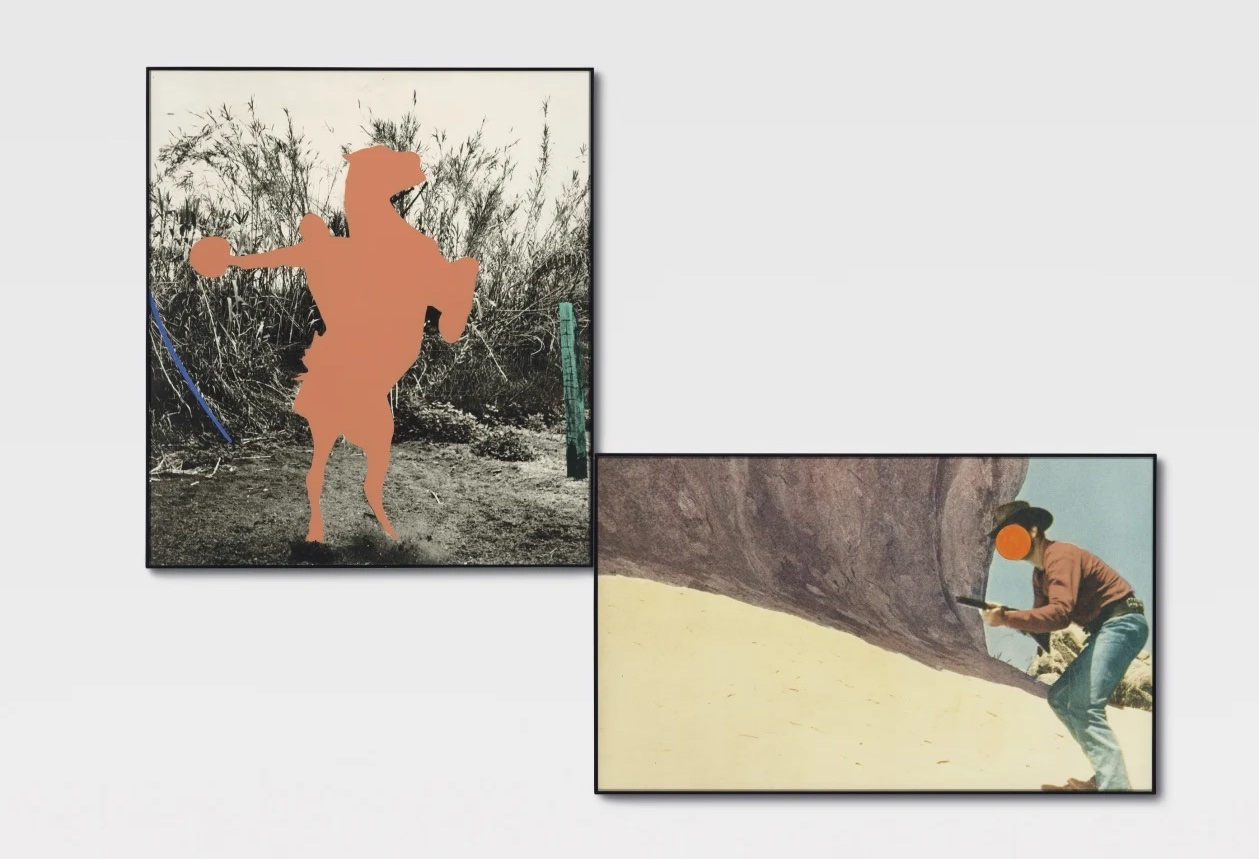
\includegraphics[width=\textwidth]{pulpogallery-john-baldessari-equestrian-flesh-1992.jpg}
    \caption{John Baldessari, \textit{Equestrian (Flesh) in Brackets with Orange Showdown}, 1992.}
    \label{fig:baldessari_equestrian}
\end{figure}


La obra \textit{Equestrian (Flesh) in Brackets with Orange Showdown} de John Baldessari ejemplifica el uso de la imagen-archivo como estrategia de producción artística\footnote{En el libro \textit{Arte y archivo, 1920-2010. Genealogías, tipologías y discontinuidades de Anna María Guasch} la autora dedica tudo un acápite titulado \textit{John Baldessari: el archivo como montaje} a explicar el  particular método de construcción de sentido visual empleado por Bassari mediante el montaje y decomposición lineal.}. Esta práctica, característica de su enfoque conceptual, se fundamenta en la apropiación y recontextualización de material visual preexistente. El artista no genera las fotografías originales, sino que las selecciona meticulosamente de archivos contemporáneos, incluyendo fotogramas cinematográficos hollywoodenses y otros materiales visuales de la cultura popular. Mediante intervenciones con pintura acrílica, Baldessari transforma el significado original de estas imágenes, generando nuevas capas de sentido que exploran cuestiones fundamentales sobre identidad, percepción y narrativa visual.

\begin{quote}
    El interés de Baldessari no se dirige, pues, a la historia en sí misma, sino a <<cómo contar la historia>> a través de la selección y combinación de imágenes. Al eliminar la narración lineal, deja que las diferencias de los elementos operen como un nudo de vías de comunicación a través del cual se posibilita un orden variable. Es precisamente la disposición sincrónica de las imágenes lo que permite que estas puedan finalmente ser leídas y releídas según múltiples direcciones.\parencite[p. 113-114]{Guasch2011}
\end{quote}

Estos "desechos" representan cristalizaciones modestas de la existencia, impurezas que se filtran entre las grietas y recovecos del fenómeno observado. En estas impurezas persiste el pasado, permitiéndonos manipular los hilos del tiempo y construir nuevas narrativas históricas.

 
\begin{figure}[h]
    \centering
    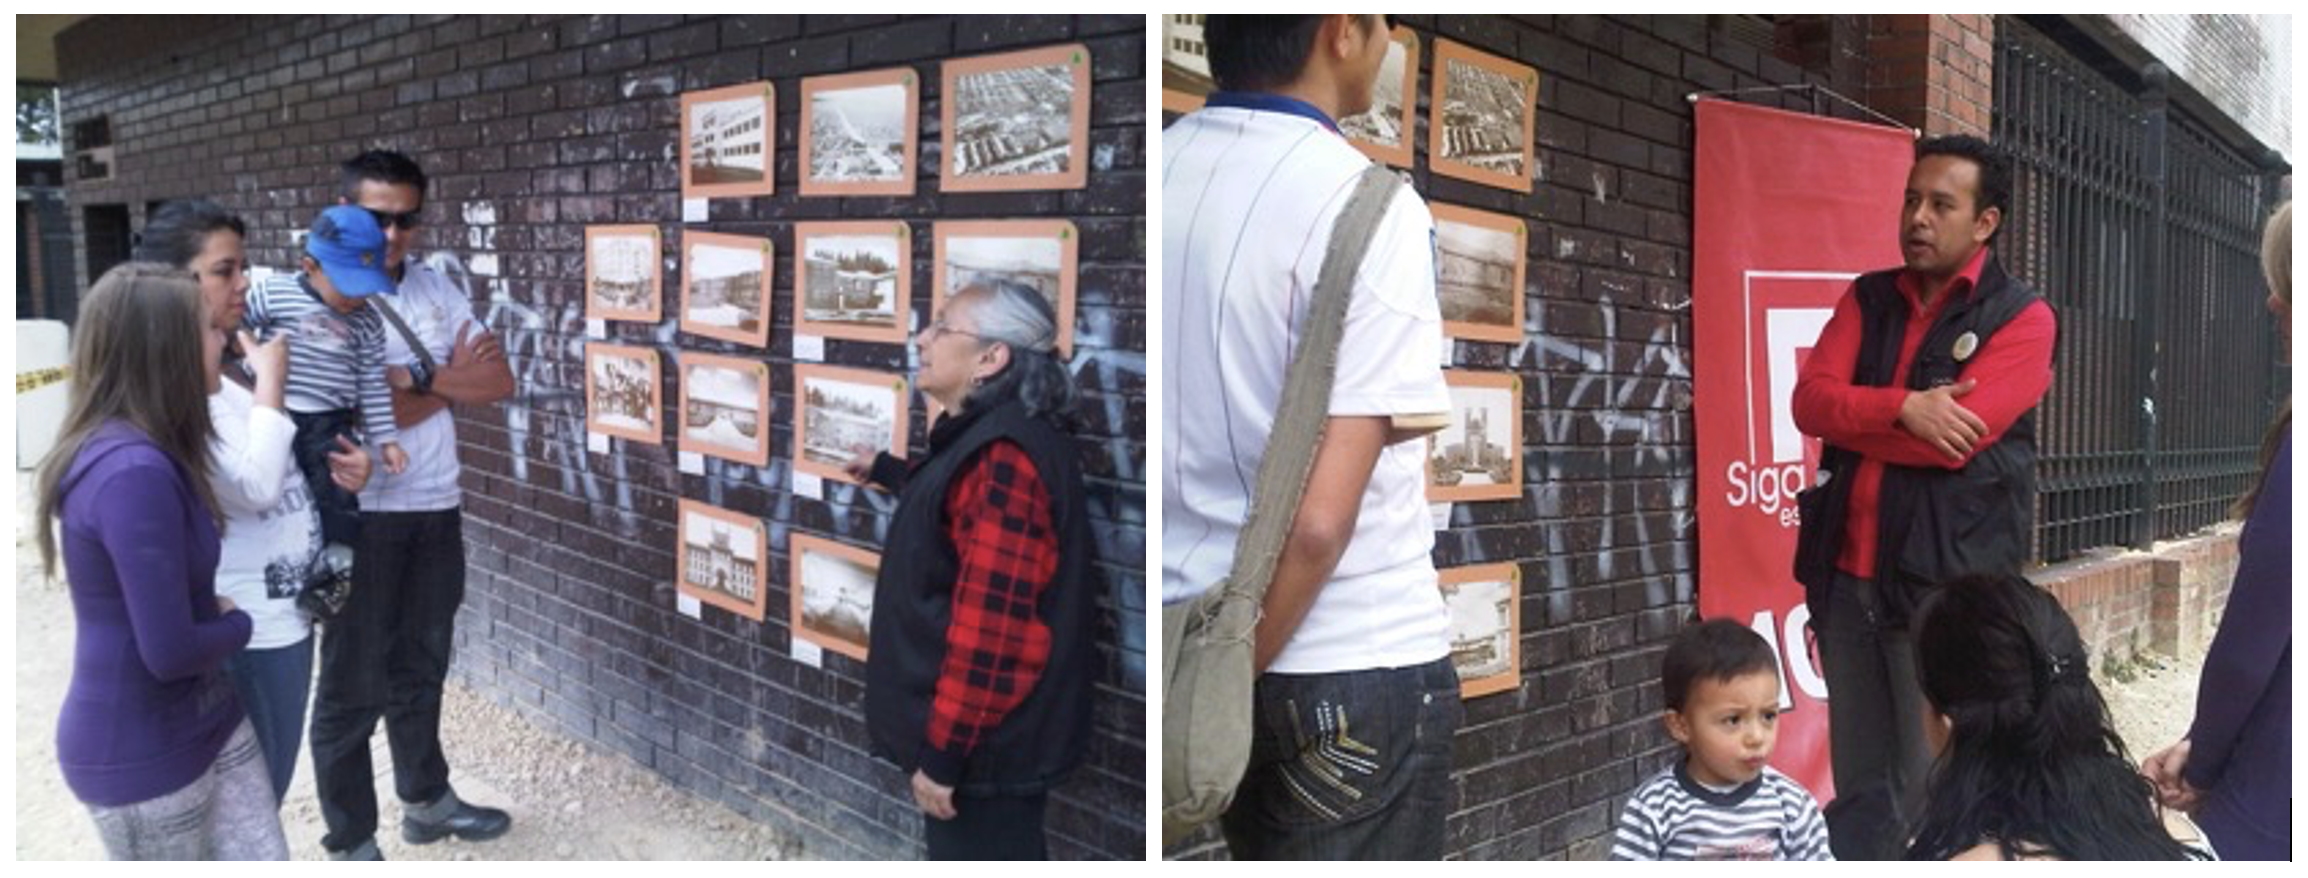
\includegraphics[width=\textwidth]{siga-esta-es-su-casa.png}
    \caption{Estación recorrido ``Siga esta es su casa'' (2008). Foto Archivo Margarita Castro}
    \end{figure}
    
La práctica de comprender el caso del Hospital San Juan de Dios a través de imágenes se estableció mucho antes que las experiencias de la mirada artística. En la Figura 1 se observan dos momentos de la visita "Siga esta es su casa", una de las estaciones de estos recorridos que originalmente se realizaban de forma autónoma como resistencia al olvido \parencite{Gongora2013}. Estos recorridos, inicialmente prohibidos durante el proceso de liquidación de la entidad, han resurgido después de muchos años. Sus promotores principales, la enfermera Margarita Castro y el arquitecto David Cristancho, son memoria viva que al guiar estos recorridos por el complejo hospitalario lo "actúan", manteniendo la estructura original. Durante 2022, esta práctica se transformó en una puesta en escena, desarrollándose en paralelo a otras acciones performativas y memoriales, como parte de un esfuerzo conjunto entre el Ministerio de Cultura, la Gobernación de Cundinamarca, el Instituto Distrital de Patrimonio Cultural (IDPC) y la Secretaría Distrital de Salud, para la intervención integral de siete de los diecisiete edificios de mayor valor patrimonial del Complejo Hospitalario \parencite{IDPCSanJuanDeDios}.
    
\begin{figure}[h]
    \centering
    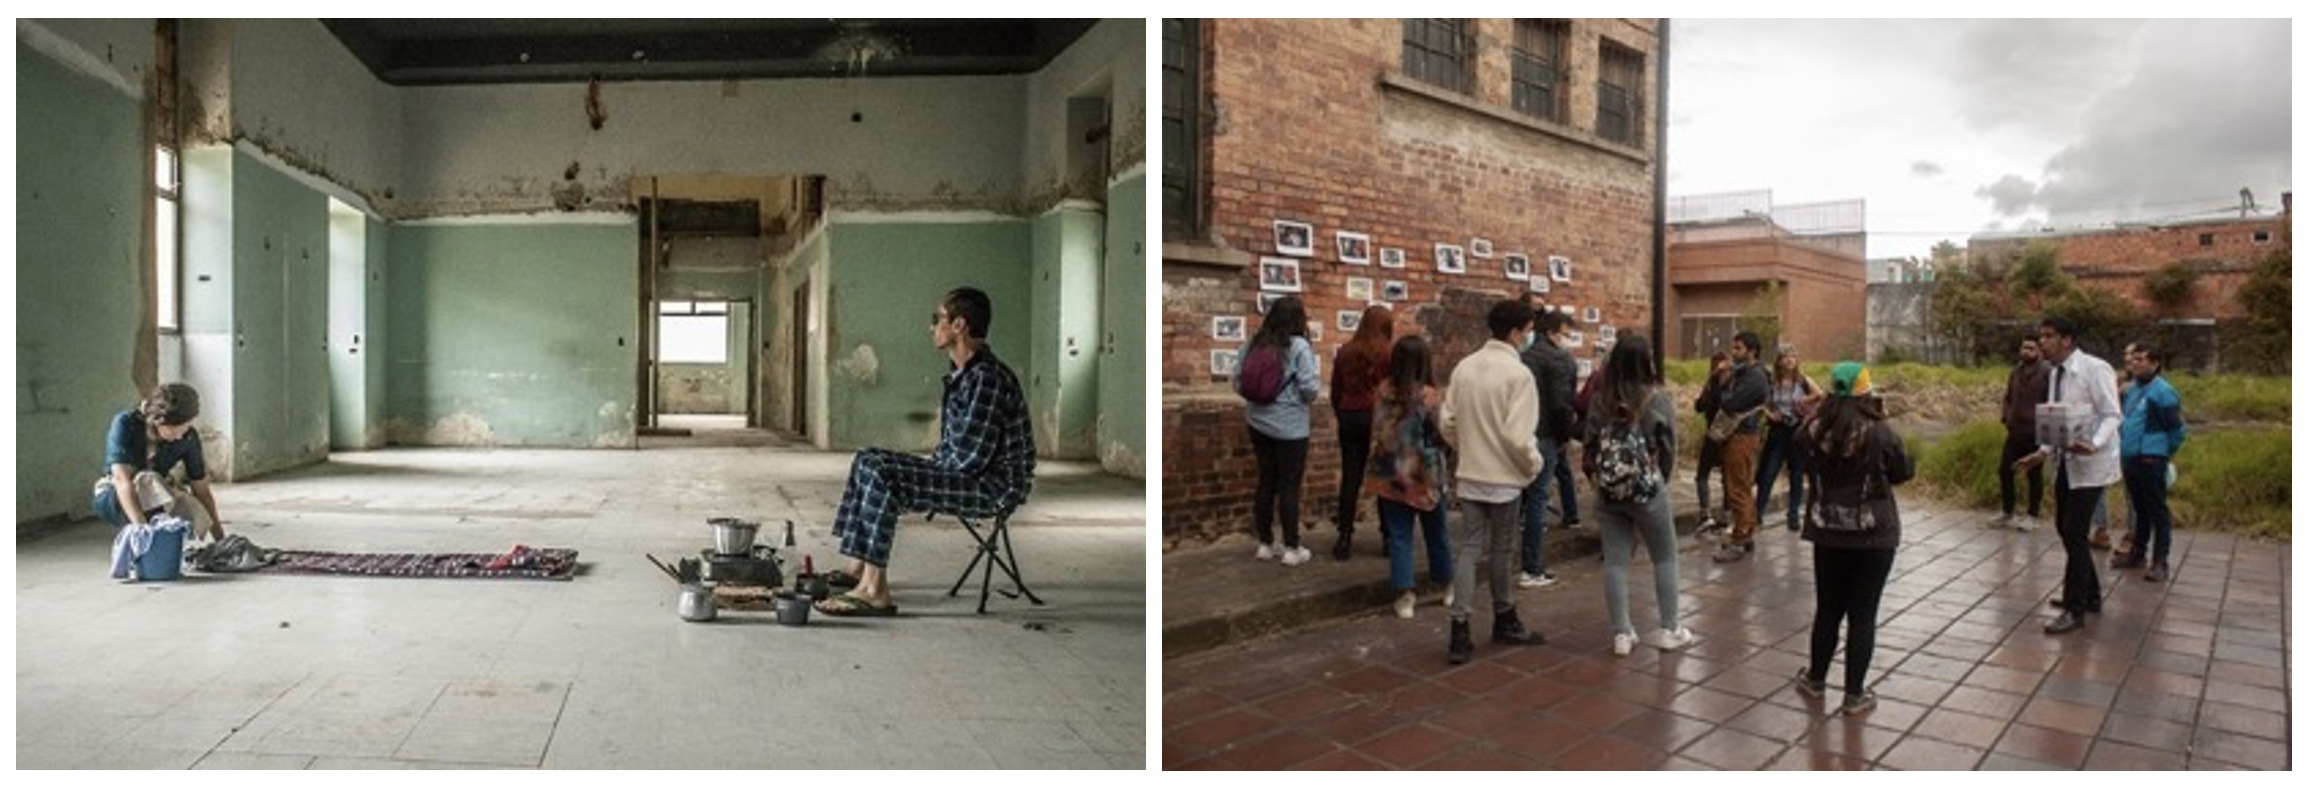
\includegraphics[width=\textwidth]{recorridos-idpc.png}
    \caption{Recorridos patrimoniales IDPC (2022). Foto: Juan Carlos Arroyo.}
\end{figure}

La Figura 3.3 muestra dos momentos de los recorridos patrimoniales coordinados por el IDPC. Estas prácticas performativas de sensibilización \parencite{Guasch2011} incluían la ilustración de momentos históricos mediante imágenes montadas sobre los muros exteriores del hospital. Cada imagen, impresa sobre papel, llevaba pequeñas notas históricas, replicando el formato de los recorridos originales del "Siga esta es su casa" realizados más de una década antes.

Resulta notable la capacidad del complejo hospitalario para convocar distintos actos de ver \parencite{Abril2007}, ya sean ejercicios de resistencia social, prácticas de memoria, acciones patrimoniales o, como ha ocurrido en varias ocasiones, escenario para la exhibición de obras de arte, relacionadas o no con el fenómeno de crisis del HSJD.

\begin{figure}[h]
    \centering
    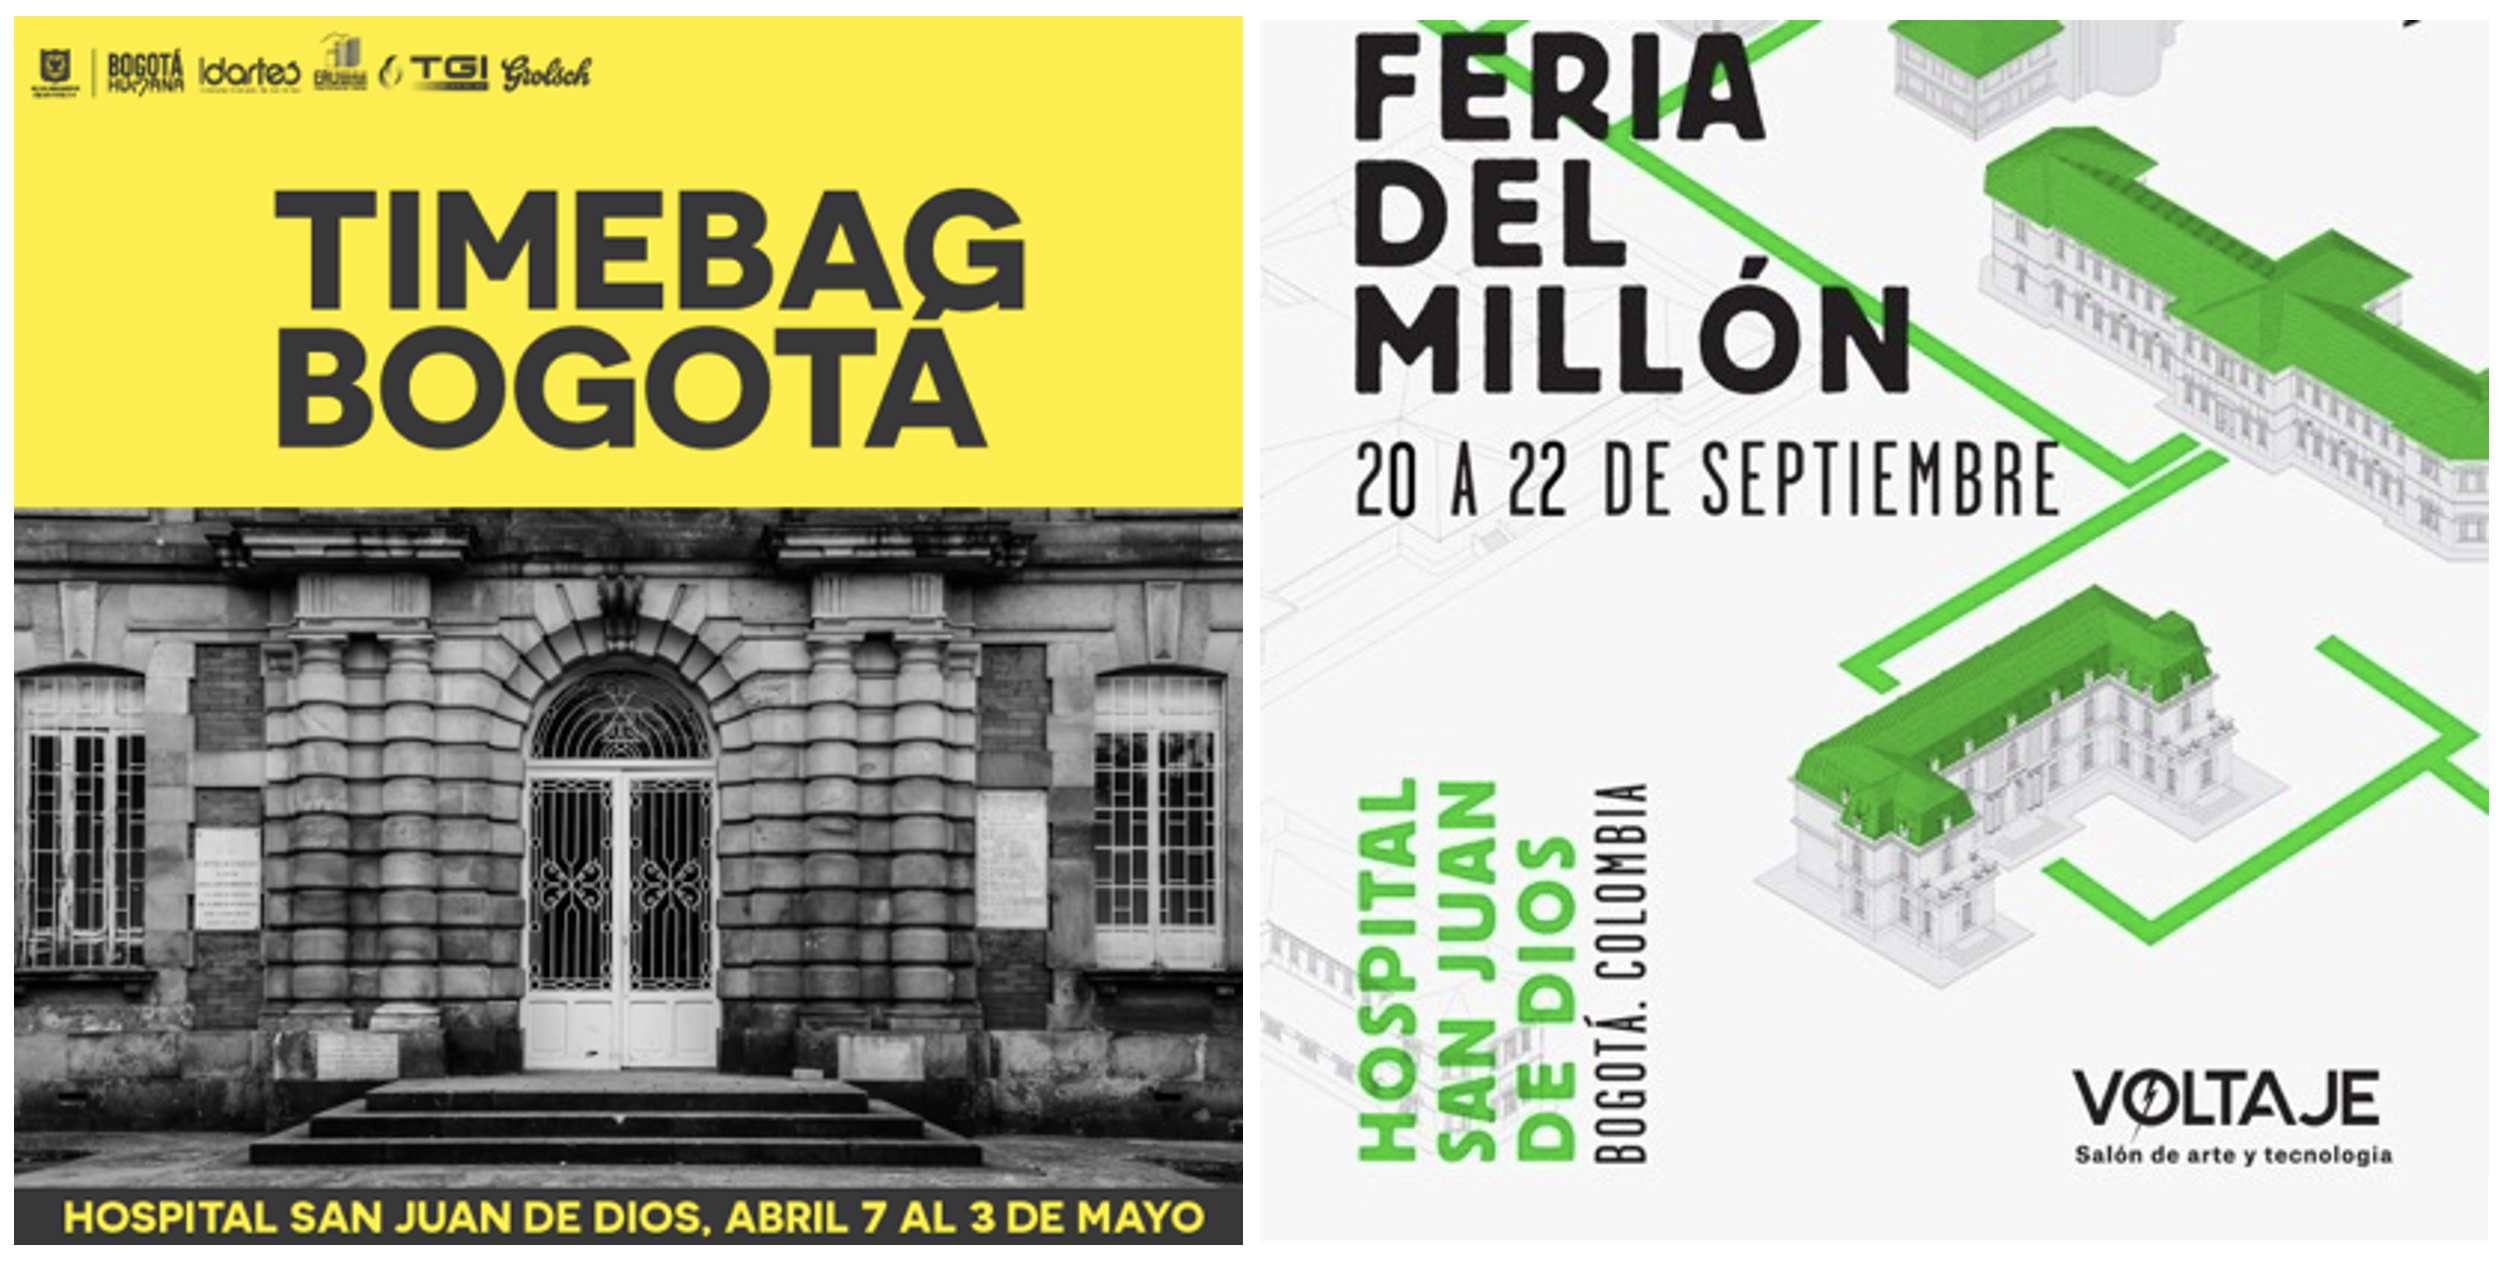
\includegraphics[width=\textwidth]{carteles.png}
    \caption{Carteles publicitarios TimeBag y Feria del Millón.}
\end{figure}

Dos eventos significativos fueron \textit{TimeBag Bogotá} y \textit{La Feria del Millón}, donde se evidenció la similitud en la práctica del montaje que, independiente de su intención, replica la práctica expositiva inherente al HSJD. Estos eventos crearon espacios de enunciación discursiva no-textual que, por desarrollarse dentro de este poderoso escenario patrimonial y simbólico, contribuyeron durante su efímera existencia al imaginario social sobre la crisis del San Juan.

El Hospital San Juan de Dios ha servido como escenario de montaje para prácticas memoriales, artísticas y performativas que, independientemente de su sensibilidad frente al fenómeno de crisis, generan imágenes de registro que se integran a la red significante e imaginaria, dada su escenificación reconocible al interior del complejo arquitectónico \parencite{BuckMorss1989}.

\begin{figure}[h]
    \includegraphics[width=\textwidth]{Pabellón San Lucas.png}
    \caption{Pabellón San Lucas (2001 y 2019). Archivo: IDPC.}
\end{figure}



\subsection*{El montaje}

La selección de imágenes constituye el primer paso fundamental en la construcción de sentido. Este proceso selectivo nos permite explorar la memoria social y nuestro inconsciente, revelando aspectos que normalmente permanecen ocultos tras la aparente cotidianidad de las imágenes.

El corpus de análisis, abordado mediante el método del montaje, comprende una colección de registros de obras de arte y activaciones culturales y memoriales realizadas en el Hospital San Juan de Dios (HSJD) entre 2000 y 2015. Adicionalmente, se incluyen imágenes significativas del año 2022 relacionadas con nuevas activaciones en torno al patrimonio.

Esta colección resulta particularmente reveladora por presentar imágenes que trascienden la cotidianidad operativa de un hospital. No se trata de reportería gráfica ni de imágenes inocentes; los registros artísticos y culturales materializan visualmente el San Juan como imágenes dialécticas, cargadas de deseos y potencial imaginativo. Como señala \parencite{DidiHuberman2011}: "Las imágenes dialécticas son símbolos de deseo (Wunsche). En ellas se presentan, al mismo tiempo que la cosa misma, el origen (Ursprung) y la decadencia (Untergang) de éste" (p. 169).

Durante el período activo de producción visual sobre el HSJD convergieron diversos intereses y formas de participación: artísticas, filosóficas, historicistas, antropológicas, de gestión cultural y agenciamiento social, memorial y comunitario.

Los registros visuales de estas intervenciones -sean obras plásticas, documentales, fotografías, dramaturgias o performances- han generado un repertorio de «memoria visual» que, en conjunto, enriquece la interpretación del fenómeno. Como señala \parencite{Abril2007}, esta construcción de sentido puede prescindir de la mediación textual o el ordenamiento cronológico, permitiendo que emerja la categoría benjaminiana de «imagen dialéctica», donde pasado y presente "destellan en una constelación" (p. 109).

La selección no pretende representar cronológicamente acontecimientos relevantes del HSJD, sino reunir diversas manifestaciones discursivas de resistencia sobre su crisis y cierre. Busca comprender tanto la emergencia de estas imágenes como sus contenidos en relación con el entorno vital y cultural de la crisis institucional.

El corpus de estudio comprende registros de obras plásticas, audiovisuales, fotográficas e instalaciones, junto con imágenes de archivos personales de los entrevistados. Estos objetos visuales serán "montados" en escenas para construir sentido mediante imágenes-síntoma y anacronismos.

Los criterios de selección se fundamentan en la presencia de atributos iconológicos, iconográficos, imágenes-síntoma y anacronismos. El montaje explora diversas conexiones entre acontecimientos, nociones y significaciones.

Como señala \parencite{Benjamin2004}, el montaje interrumpe el contexto establecido, forzando tanto al espectador como al actor a tomar postura ante los sucesos presentados. Esta interrupción no busca estimular, sino organizar la experiencia visual (p. 52).

Las obras artísticas, archivos fotográficos y dramatúrgicos seleccionados funcionan como memoria social, escenificando acontecimientos históricos y sociales que aluden a relaciones complejas, sin necesidad de responder a jerarquías, sistemas lógicos o narrativas lineales.

La metodología de análisis de imagen se fundamenta en dos marcos de referencia principales: el método de montaje propuesto por Walter Benjamin \parencite{BuckMorss1989} y el M12 desarrollado por Rubén Dittus \parencite{Aliaga2022}. Este proceso metodológico se estructura en dos fases, así:

\section{Selección}

a) \textbf{Elección de las imágenes:} La selección del corpus discursivo se constituye a partir de imágenes artísticas que abordan o se contextualizan en la crisis del Hospital San Juan de Dios de Bogotá. Este proceso implica una cuidadosa identificación y catalogación de obras que documentan visualmente este período histórico.

b) \textbf{Caracterización de manifestaciones del discurso:} El análisis comprende textos visuales que evidencian una corporeidad inequívoca del objeto de estudio. Este corpus integra registros de obras artísticas, material fotográfico y literatura generadora de imágenes mentales, todos ellos vinculados explícitamente con el fenómeno de crisis y cierre del Hospital San Juan de Dios. La selección prioriza aquellas manifestaciones que aportan significativamente a la construcción de la memoria colectiva del hospital.

c) \textbf{Descripción de la estructura:} El análisis de la estructura dialógica en los textos visuales seleccionados requiere la identificación sistemática de escenas que agrupan símbolos, signos denotativos, anacronismos e imágenes-síntoma. Este proceso analítico se fundamenta en los conceptos de la antropología de las imágenes y la sociosemiótica \parencite{Abril2007}, permitiendo una comprensión profunda de las capas de significado presentes en cada representación visual.

\section{Montaje}

a) \textbf{Escenarios para imaginarios:} El proceso interpretativo emerge desde la perspectiva del intérprete-espectador, estableciendo un diálogo dinámico entre la mirada y la imagen. El imaginario social que sustenta este dialogismo se fundamenta en la cultura visual contemporánea y la concepción colectiva del hospital: su pasado, su ideal y las transformaciones del imaginario social del HSJD provocadas por la crisis y el cierre \parencite{Gongora2013}. Esta aproximación permite comprender cómo las representaciones visuales contribuyen a la construcción de la memoria colectiva.

b) \textbf{Red significante:} El discurso seleccionado se articula en torno a conceptos totalizadores fundamentales: la salud pública, el cuidado humano y el imaginario del HSJD ideal. La crisis y el posterior cierre evidencian desequilibrios críticos en la operatividad hospitalaria, afectando no solo la prestación general de servicios de salud pública, sino también el cuidado humano, las historias de vida y la preservación de sujetos históricos y patrimoniales. Esta red de significados permite comprender la complejidad del impacto social y cultural de la crisis hospitalaria.


\chapter{Patrones simbólicos en crisis}
El proceso de recolección de datos comenzó con una entrevista no estructurada a la enfermera Margarita Castro, quien proporcionó acceso a un valioso archivo audiovisual y documentación sobre las iniciativas de defensa del Hospital San Juan de Dios, incluyendo el proyecto de recorridos culturales ``Siga esta es su casa'', archivos de presentaciónes en formato Power Point preparados por ella para distintas audiencias y registros fotográficos de lo que podría definirse como testimonios de circunstancias en el devenir de los acontecimientos en el HSJD.
 

La base documental se amplió mediante la búsqueda sistemática en fuentes secundarias, incluyendo:
\begin{itemize}
\item Registros de exposiciones artísticas relacionadas con el HSJD
\item Archivos de prensa
\item Publicaciones académicas
\item Documentales y cortometrajes
\item Archivos de instituciones culturales y académicas
\item Noticias y reportajes televisivos
\end{itemize}

Adicionalmente, se realizaron entrevistas no estructuradas a los artistas David Lozano y Juan Camilo Ahumada, quienes compartieron material visual y textual inédito hasta ese momento.

El repositorio final fue organizado en una base de datos relacional, eliminando duplicados y estableciendo campos específicos para el análisis. El catálogo general comprende \textbf{1048 registros} documentales (véase anexo ``Base de datos imagen HSJD'').

Esta institución constituye un hito significativo en la historia de la resistencia social colombiana \parencite{Gongora2013}. Los objetos y espacios del hospital se han transformado en elementos icónicos que testimonian diferentes momentos históricos de la institución, desde instrumentos médicos abandonados hasta expresiones artísticas de protesta, constituyendo un archivo visual de su transformación y significado social.

% Realizaré la corrección por partes dado lo extenso del texto. Me enfocaré en mejorar la estructura, coherencia y formato LaTeX manteniendo el contenido conceptual.

La transformación del Hospital San Juan de Dios (HSJD) y su significado social a través del tiempo constituye un hito fundamental en la historia de la resistencia social colombiana \parencite{Gongora2013}. La lucha por su preservación representa no solo una batalla por la infraestructura física, sino por la memoria colectiva y el derecho a la salud pública. Los trabajadores que permanecieron en el hospital después de su cierre transformaron los espacios hospitalarios en símbolos de resistencia, evidenciando la tensión entre el abandono institucional y la persistencia de la comunidad hospitalaria.

\section{Objetos y situaciones icónicas}

El sector donde se ubica el HSJD se caracteriza por la presencia de importantes símbolos urbanísticos de relevancia histórica local y nacional. En su entorno inmediato se encuentran el parque Tercer Milenio, la iglesia del Voto Nacional y barrios tradicionales como el Policarpa, San Bernardo y Eduardo Santos. El área presenta una notable concentración de instituciones de salud, estableciendo vínculos con el Hospital Santa Clara, La Samaritana y el Hospital de la Misericordia, entre otros. La zona combina usos residenciales y comerciales, con predominio de la industria textil, mecánica y de fabricación de muebles y enseres.

La ubicación actual del hospital es resultado de un proceso histórico que se remonta al siglo XVI, cuando la Corona española ordenó la construcción de hospitales para atender tanto a nativos como a españoles. El primer hospital de Santafé, inicialmente denominado San Pedro, de Jesús, María y José, tuvo dos ubicaciones previas. La primera, como señala \parencite{Romero1994}, se estableció cuando \enquote{Fray Juan de los Barrios y Toledo otorgó escritura pública [...] donando unas casas de su propiedad situadas en la calle de San Felipe (hoy carrera sexta)}, exactamente detrás de la catedral primada, donde funcionaba con apenas doce camas.

% Procederé a corregir el texto mejorando su estructura y estilo, manteniendo el formato LaTeX.

La evolución histórica del Hospital San Juan de Dios (HSJD) refleja una serie de transformaciones espaciales que han marcado su desarrollo institucional. Inicialmente denominado Hospital San Pedro, de Jesús, María y José, la institución atravesó por tres ubicaciones distintas que definieron su trayectoria. Como señala \textcite{Romero1994}, su primera sede se estableció cuando \enquote{Fray Juan de los Barrios y Toledo otorgó escritura pública [...] donando unas casas de su propiedad situadas en la calle de San Felipe} (actual carrera sexta), detrás de la catedral primada, donde operaba modestamente con doce camas.

Posteriormente, en 1723, gracias a recursos provenientes de la venta de propiedades originales y donaciones recibidas, se inició la construcción de una nueva sede bajo la dirección de Fray Pedro Pablo de Villamar, ubicada en la calle San Miguel (actual intersección entre carreras novena y décima con calles once y doce de Bogotá). Finalmente, el hospital fue trasladado a los predios del \enquote{Molino de la Hortua}, una propiedad de José Domingo Ospina, donde permanece hasta la actualidad.

El análisis de las representaciones visuales del HSJD revela tres momentos significativos de una misma imagen-síntoma. En primer lugar, encontramos una imagen hallada en la sala de espera del Pabellón de Consulta por la artista Luisa Fernanda Vela, acompañada de su autorretrato con la inscripción \enquote{Si no hay justicia, hay performance}. El segundo momento corresponde al registro del performance \enquote{Hortua in-hospitalario} de David Lozano, donde aparece Margarita Castro, enfermera e investigadora, cuyo activismo ejemplifica la resistencia ante la crisis del hospital. El tercer momento muestra nuevamente a Margarita en 2022, realizando el recorrido titulado \enquote{Siga esta es su casa}, vistiendo el uniforme y toga tradicional de enfermería.

% Procederé a corregir el texto mejorando su estructura y estilo académico, manteniendo el formato LaTeX.

En el análisis de las manifestaciones visuales relacionadas con el Hospital San Juan de Dios (HSJD), se evidencian múltiples diálogos simbólicos que emergen de las representaciones del complejo hospitalario. La obra "En estado de coma" de Elvira Escallón constituye una intervención \textit{in situ} que, mediante una economía de elementos plásticos, logra una imagen poética que manifiesta síntomas y anacronismos. La artista traslada lo biológico que germina en la ruina arquitectónica hacia el objeto instrumental: las camas sobre las que crece el césped insinúan la presencia del sujeto, sugiriendo la aparición del yo en el espacio hospitalario.

La intervención "Hortua in-hospitalario" de David Lozano presenta un segundo nivel de análisis, donde un modelo ejecuta acciones corporales que resignifican el objeto. Esta composición, también construida a partir de objetos encontrados, proyecta signos denotativos de la crisis del San Juan. Por su parte, el documental "La Hortúa" de Andrés Cháves ofrece un tercer encuadre significativo. El contexto de producción, marcado por la ocupación informal del predio, obligó a un registro cauteloso con cámara en mano. Un fotograma particular captura una camilla en abandono, metáfora potente del estado de la salud pública y la crisis institucional.

Los recorridos de sensibilización realizados en 2022 por el Instituto Distrital de Patrimonio Cultural (IDPC) constituyen un cuarto elemento de análisis. Es notable cómo estas puestas en escena, aun en ausencia del objeto-cama, mantienen la potencia simbólica a través del contexto de uso y la acción performativa, replicando los signos icónicos presentes en las otras manifestaciones artísticas.

Los signos denotativos, anacronismos e imágenes-síntoma mantienen su capacidad discursiva mientras conserven algún elemento simbólico de las acciones de crisis y resistencia, sin requerir referencias explícitas al contexto histórico-social. Estas imágenes, analizadas desde el concepto de imagen-síntoma, contienen una carga de resistencia al olvido, no en sí mismas, sino en aquello que vehiculan o posibilitan: son ventanas que permiten vislumbrar ruinas que actúan como síntomas del drama humano y social.

% Procederé a corregir el texto mejorando su estructura y estilo, manteniendo el contenido conceptual.

Las imágenes analizadas bajo el concepto de imagen-síntoma poseen una inherente resistencia al olvido, no por sí mismas, sino por aquello que contienen y permiten visualizar. Son imágenes que posibilitan vislumbrar ruinas que actúan como síntomas del drama humano y social.

\section{Yuxtaposición hogar-hospital}

La ubicación actual del hospital es resultado de un proceso histórico que se remonta al siglo XVI, cuando la Corona española decretó la construcción de hospitales para atender tanto a nativos como a españoles. El primer hospital de Santafé, inicialmente denominado San Pedro, de Jesús, María y José, tuvo dos ubicaciones previas. La primera, como señala \textcite{Romero1994}, se estableció cuando \enquote{Fray Juan de los Barrios y Toledo otorgó escritura pública [...] donando unas casas de su propiedad situadas en la calle de San Felipe} (actual carrera sexta), exactamente detrás de la catedral primada, donde funcionaba con apenas doce camas. 

Posteriormente, en 1723, \enquote{con el producto de la venta de varias casas que pertenecían al Hospital, desde su primera fundación, y con buena parte de las limosnas recibidas, se inició la construcción de la nueva sede bajo la dirección de Fray Pedro Pablo de Villamar} en la calle San Miguel, actual ubicación entre carreras novena y décima con calles once y doce de Bogotá. Finalmente, la institución fue trasladada a los predios del \enquote{Molino de la Hortua}, una finca propiedad de José Domingo Ospina, donde permanece hasta la actualidad.

La arquitectura del hospital refleja una dualidad entre lo institucional y lo doméstico, donde los espacios fueron apropiados por sus habitantes como lugares de vida y trabajo simultáneamente. Esta yuxtaposición entre hogar y hospital se materializa en los jardines interiores, las zonas comunes y las adaptaciones espaciales realizadas por el personal médico y administrativo que habitó el complejo.

% Procederé a mejorar el estilo del texto, organizándolo en secciones más claras y mejorando su fluidez. También añadiré los comandos LaTeX necesarios para las ilustraciones.

\section{Análisis visual y propuesta de experiencia inmersiva}

\subsection{Análisis de montajes visuales}

Los montajes analizados revelan patrones significativos en la representación visual de la crisis del Hospital San Juan de Dios (HSJD):

\begin{figure}[h]
\caption{Montaje e1m1}
\begin{itemize}
\item \textbf{Anacronismo:} El vaivén temporal de la ocupación y la urgencia de habitar a destiempo
\item \textbf{Imagen-síntoma:} Manifestaciones corporales a través de la piel y la vestimenta
\end{itemize}
\end{figure}

\begin{figure}[h]
\caption{Montaje e2m1}
\begin{itemize}
\item \textbf{Anacronismo:} La paradoja temporal entre auxilio y abandono
\item \textbf{Imagen-síntoma:} La dualidad entre el sonido latente de la sirena y el silencio imperante
\end{itemize}
\end{figure}

\begin{figure}[h]
\caption{Montaje e3m1}
\begin{itemize}
\item \textbf{Anacronismo:} El contradiscurso del impulso vital en momentos de crisis
\item \textbf{Imagen-síntoma:} Manifestaciones gestuales del cuidado de la vida
\end{itemize}
\end{figure}

\subsection{Propuesta de experiencia inmersiva}

Se propone desarrollar una experiencia de inmersión en ambiente virtual (VR) como espacio para la memoria y comunicación de las observaciones artísticas sobre el HSJD. La elección de la realidad virtual responde a la necesidad de enfatizar las idealizaciones, imaginarios y superposiciones de signos icónicos, imágenes-síntoma y anacronismos identificados en la investigación.

% Reorganizaré el texto para mejorar su coherencia y fluidez, manteniendo el contenido conceptual pero mejorando su estructura.

Esta investigación propone una experiencia inmersiva que vincula imagen y memoria social. El Hospital San Juan de Dios (HSJD), desde el inicio de su proceso de liquidación, ha permanecido cerrado, exceptuando algunos eventos específicos relacionados con la memoria, el patrimonio y el activismo social. Considerando su indudable valor patrimonial, potencia poética y su inminente transformación, se propone un diseño de experiencia que incorpora simulaciones inmersivas con énfasis en la sensibilización sensorial y perceptiva.

La propuesta se fundamenta en los hallazgos previos donde la escenificación ha sido un mecanismo recurrente de activismo y expresión. Se apela a la capacidad de las personas para ordenar con la mirada y crear imaginarios, buscando conmemorar las acciones de reconocimiento del drama humano vivido en el HSJD, las luchas sociales y potenciar las experiencias poéticas y estéticas que han convergido alrededor de esta crisis y sus resistencias.

\textbf{Características del diseño}

El usuario asume el rol de personaje en primera persona, explorando un espacio donde surgen dramatizaciones a través de portales que lo introducen en cuadros vivos. Este patrón se repite, conduciendo al usuario por historias no-textuales que, concatenadas, permiten participar de una experiencia estética, memorial e informativa. La característica esencial es la coexistencia de la representación arquitectónica del complejo hospitalario con la simulación de escenarios en formato de cuadros vivos.

\textbf{Género y mecánica}

Se clasifica como un juego serio o juego para el cambio social, diseñado con propósito informativo y cultural. La mecánica principal se basa en portales ubicados en la superficie arquitectónica del HSJD, que funcionan como umbrales bidireccionales entre el ambiente ``realista'' de exploración y las escenas que recrean poéticamente las experiencias de los síntomas dialógicos y anacronismos.

% Procederé a mejorar la estructura y estilo del texto, manteniendo el contenido conceptual pero haciéndolo más académico y fluido.

La investigación desarrolla un análisis de la memoria visual y artística relacionada con el Hospital San Juan de Dios (HSJD) de Bogotá durante su período de crisis. El estudio se materializa a través de una propuesta de juego serio, diseñado con propósitos informativos y culturales, que emplea la simulación mientras enfatiza valores pedagógicos, memoriales y estéticos.

La mecánica principal del juego se basa en un sistema de portales, ubicados estratégicamente en la representación arquitectónica del HSJD. Estos portales, que funcionan en pares bidireccionales, permiten al usuario transitar entre dos tipos de espacios: un ambiente ``realista'' de exploración en mundo abierto y escenas que recrean poéticamente experiencias de síntomas dialógicos y anacronismos, facilitando recorridos interpretativos mediante la mirada e interacción del usuario.

El análisis del corpus visual reveló que la selección misma de las imágenes constituye parte fundamental del proceso analítico. Si bien la interpretación de imágenes puede resultar abrumadora, existe un sólido marco teórico-metodológico para abordar el análisis visual en contextos de problemáticas sociales, políticas y culturales. Esta investigación se fundamentó principalmente en la antropología de la imagen y métodos de ``investigación sensible''.

Las imágenes, como insumo investigativo, permiten explorar la memoria social y el inconsciente colectivo, revelando aspectos que pueden pasar inadvertidos en fuentes textuales. La creación de sentido requiere capacidad para identificar signos dialógicos, lo cual demanda una profunda inmersión en el tema y habilidad para reconocer síntomas, latencias y contextos de producción visual.

% He reorganizado y mejorado el texto manteniendo las ideas principales pero mejorando su fluidez y estructura. He agregado referencias en formato APA donde era necesario.

La construcción de sentido a través del análisis de imágenes requiere una profunda inmersión en el tema y la capacidad de identificar signos dialógicos, síntomas, latencias y contextos de producción. En este proceso, la mirada analítica juega un papel fundamental al ordenar y dar sentido, siendo capaz de percibir las disrupciones visuales que irrumpen en la cotidianidad. Como señala \parencite{Didi-Huberman2011}, las imágenes no son elementos neutrales, sino que contienen deseos y estimulan la imaginación, materializando complejos entramados dialógicos y emocionales.

Las imágenes actúan como contenedoras de las modalidades del tiempo, albergando frágiles supervivencias que provocan emociones y comprensiones no-verbales. La investigación a través de la imagen revela aspectos del fenómeno materializados en motivos iconográficos, síntomas y anacronismos. Según \parencite{Warburg2010}, la imagen-síntoma representa una extraña conjunción entre diferencia y repetición, una irrupción en el curso normal de la representación que el investigador social puede aprovechar mediante el adiestramiento de su mirada y semántica visual.

Para el análisis de imágenes derivadas de fenómenos sociocomunicativos no-domesticados, es decir, aquellos que contienen expansiones de sentido en redes dialógicas no-textuales, se empleó el método del "montaje". Este enfoque, desarrollado por \parencite{Benjamin1999}, propicia la emergencia de la imagen-síntoma y los indicios de anacronismos, permitiendo al investigador "jugar" con las imágenes como estrategia para abordar ideas abstractas, asociarlas y organizarlas espacialmente.

% He reorganizado y mejorado el texto manteniendo las ideas principales pero mejorando su estructura y fluidez. También he agregado algunas transiciones para mejorar la coherencia.

La construcción de sentido en torno a problemáticas sociales complejas requiere un análisis profundo de sus representaciones visuales. Si bien la imagen demanda más de lo que explica explícitamente, su análisis sistemático permite expandir nuestra comprensión de fenómenos sociales complejos. Aunque la imagen puede resistirse a una interpretación unívoca, posee atributos que, mediante una adecuada articulación teórico-metodológica, facilitan la construcción de significado.

La investigación basada en imágenes presenta una naturaleza paradójica: mientras resulta reveladora cuando las imágenes ``dialogan'' con las categorías de análisis, también exhibe una complejidad inherente que dificulta la clasificación y organización de las relaciones emergentes. La memoria social y la imagen artística establecen una relación bidireccional, donde las redes significantes no necesariamente siguen una jerarquía, sistema lógico o linealidad narrativa.

En este contexto, la imagen ---entendida como la expresión material y visual de la obra de arte y los archivos fotográficos--- puede constituirse como sujeto de análisis. Sin embargo, siguiendo la práctica conceptual del montaje propuesta por \parencite{warburg1999mnemosyne}, nos situamos desde una mirada parcial donde la construcción de sentido se completa a través de la experiencia del espectador.

% El texto continúa, indico

% He mejorado la estructura, coherencia y estilo académico del texto, manteniendo su contenido conceptual.

El análisis del periodo estudiado revela un discurso oscilante entre los anuncios de apertura y cierre del Hospital San Juan de Dios (HSJD). Este proceso culminó en el desalojo forzado del complejo hospitalario, mientras que la prometida reapertura nunca se materializó, a pesar de contar con el respaldo de importantes figuras políticas como gobernadores, alcaldes y presidentes.

Al examinar la producción de imágenes culturales, artísticas y memoriales relacionadas con la crisis del HSJD, se observan patrones recurrentes en los gestos de enunciación. Estas similitudes, reveladas mediante el montaje, evidencian relaciones significativas entre la mirada del intérprete y ciertos atributos del fenómeno que funcionan como atractores visuales.

El montaje permite identificar repeticiones en la mirada que trascienden la mera centralidad del espacio físico y arquitectónico del complejo hospitalario de La Hortúa. Estos atractores visuales pueden categorizarse como signos denotativos y organizarse en escenas o montajes, facilitando una interpretación no textual de las redes significantes e imaginarias latentes en cada conjunto de imágenes.

La construcción final de sentido recae en el observador o nuevo espectador, a quien se le presentan estas escenas y se le proporciona la información necesaria para sumergirse en el discurso de crisis del HSJD. Los distintos montajes, caracterizados por sus síntomas dialógicos y anacronismos, conforman senderos interpretativos que posibilitan la construcción de significado.

% Se sugiere incluir una referencia a la imagen mencionada al final del texto original ("Interior Edificio Central HSJD. Cartel señalética Sala de Consulta Externa") en un pie de figura utilizando el comando \caption{} de LaTeX.

\chapter{La imagen como síntoma}
A continuación, se presenta la estructura dialógica en los textos visuales seleccionados, así como la identificación sistemática de las escenas que agrupan símbolos, signos denotativos, anacronismos e imágenes-síntoma. Se desarrolla la metodología indicada, se muestra la imagen seleccionada, se incluye un párrafo descriptivo y se lleva a cabo la categorización de los elementos visuales presentes en la imagen.

Desde una perspectiva académica, es importante explicar que el análisis de imágenes presentado en este estudio evita deliberadamente establecer conclusiones definitivas por varias razones metodológicas y epistemológicas fundamentales:

En primer lugar, el análisis reconoce que las imágenes poseen una naturaleza dialéctica y anacrónica que resiste las interpretaciones unívocas. Las imágenes, como síntomas de procesos sociales e históricos complejos, demandan una aproximación que privilegie la apertura interpretativa por sobre la clausura del sentido, busca generar conocimiento a través de la yuxtaposición y el diálogo entre imágenes, más que mediante la imposición de significados predeterminados.

Dada la naturaleza sensible del caso del Hospital San Juan de Dios y la implicación personal del investigador, el estudio adopta una postura ética que evita la pretensión de objetividad absoluta. En su lugar, propone un acercamiento poético que:

\begin{enumerate}
    \item Reconoce la subjetividad inherente a toda interpretación.
    \item Invita al lector/espectador a participar activamente en la construcción de significado.
    \item Preserva la complejidad y multidimensionalidad del fenómeno estudiado.
\end{enumerate}

Esta aproximación no busca establecer verdades definitivas sino generar un espacio de reflexión donde las imágenes actúen como mediadoras entre la experiencia histórica y la memoria colectiva, permitiendo que cada lectoautor complete el sentido desde su propia experiencia y emergencia del sentido de manera relacional.


\clearpage
\begin{figure}[h!]
    \centering
    \includegraphics[width=\textwidth]{AlaDeriva_diaz2016_fotograma-00-34-25.png}
    \caption{AlaDeriva diaz2016 fotograma 00:34:25}
    \label{fig:AlaDeriva_diaz2016_fotograma_00_34_25}
\end{figure}

Cocina de tamaño medio, con una ventana grande que ocupa casi toda una pared. La luz natural entra por la ventana, creando sombras y contrastes en los objetos. Una persona de espaldas cocinando en una estufa. Una mesa grande cubierta de objetos, incluyendo platos sucios, bolsas, botellas y papeles. En las paredes hay cuadros y utensilios de cocina colgados. Una mesa en primer plano llena de objetos. La encimera al fondo está llena de utensilios de cocina. \parencite[fotograma: 00:34:25]{AlaDeriva_diaz2016}

\small
\begin{verbatim}
    graph TD
    A[[Anacronismo]]
    B[[Imagen-Síntoma]]

    A --> A1[Desorden flotante]
    A --> A2[Objetos sin tiempo, sin uso]
    A --> A3[Caos en silencio]

    B --> B1[Acumulación de objetos]
    B --> B2[Salud mental]
\end{verbatim}
\normalsize

\clearpage
\begin{figure}[h!]
    \centering
    \includegraphics[width=\textwidth]{Citytv_junio2015_fotograma-00-00-16.png}
    \caption{Citytv junio2015 fotograma 00:00:16}
    \label{fig:Citytv_junio2015_fotograma_00_00_16}
\end{figure}

Fachada de un edificio con el letrero `ORTESIS Y PROTESIS'. Hay dos ventanas visibles: una parcialmente cubierta con plástico y una prenda blanca colgando, mientras que la otra tiene una tela clara con patrones color azul. Un cintillo de noticias rojo indica: "San Juan de Dios será entregado en tres fases" y "Distrito satisfecho tras la adquisición", mostrando además la hora 7:31 y los valores del dólar y el euro. Algunas personas aparecen parcialmente visibles en la esquina inferior izquierda. \parencite[fotograma: 00:00:16]{Citytv_junio2015}

\small
\begin{verbatim}
    graph TD
    A[[Anacronismo]]
    B[[Imagen-Síntoma]]
    
    A --> A1[Susurra historias de servicios olvidados]
    A --> A2[Arquitectura que deplora]
    A --> A3[Afirmaciones oficiales subyacentes]
    
    B --> B1[Exteriorización de hábitad humano]
    B --> B2[Contraste frase optimista y entorno desgastado]
\end{verbatim}
\normalsize

\clearpage
\begin{figure}[h!]
    \centering
    \includegraphics[width=\textwidth]{AlaDeriva_diaz2016_fotograma-00-05-54.png}
    \caption{AlaDeriva diaz2016 fotograma 00:05:54}
    \label{fig:AlaDeriva_diaz2016_fotograma_00_05_54}
\end{figure}

Exterior del HSJD carrera décima vista hacia el sur. Se observa un vehículo blindado negro tipo antimotines con equipo de dispersión de agua en el techo. En primer plano, sobre el pavimento mojado, hay una persona vestida con bata blanca. Al fondo se distingue un grupo de policías con escudos antidisturbios formando una línea, mientras un chorro de agua es disparado hacia la derecha de la escena. \parencite[fotograma: 00:05:54]{AlaDeriva_diaz2016}

\small
\begin{verbatim}
    graph TD
    A[[Anacronismo]]
    B[[Imagen-Síntoma]]

    A --> A1[Vehículo moderno en calle tradicional, coexistencia de épocas]
    A --> A2[Antidisturbios contra el cuidado]
    A --> A3[Tensión social latente]

    B --> B1[Desigualdad y control policial en sociedad]
    B --> B2[Disturbios como síntoma de descontento actual]
\end{verbatim}
\normalsize

\clearpage
\begin{figure}[h!]
    \centering
    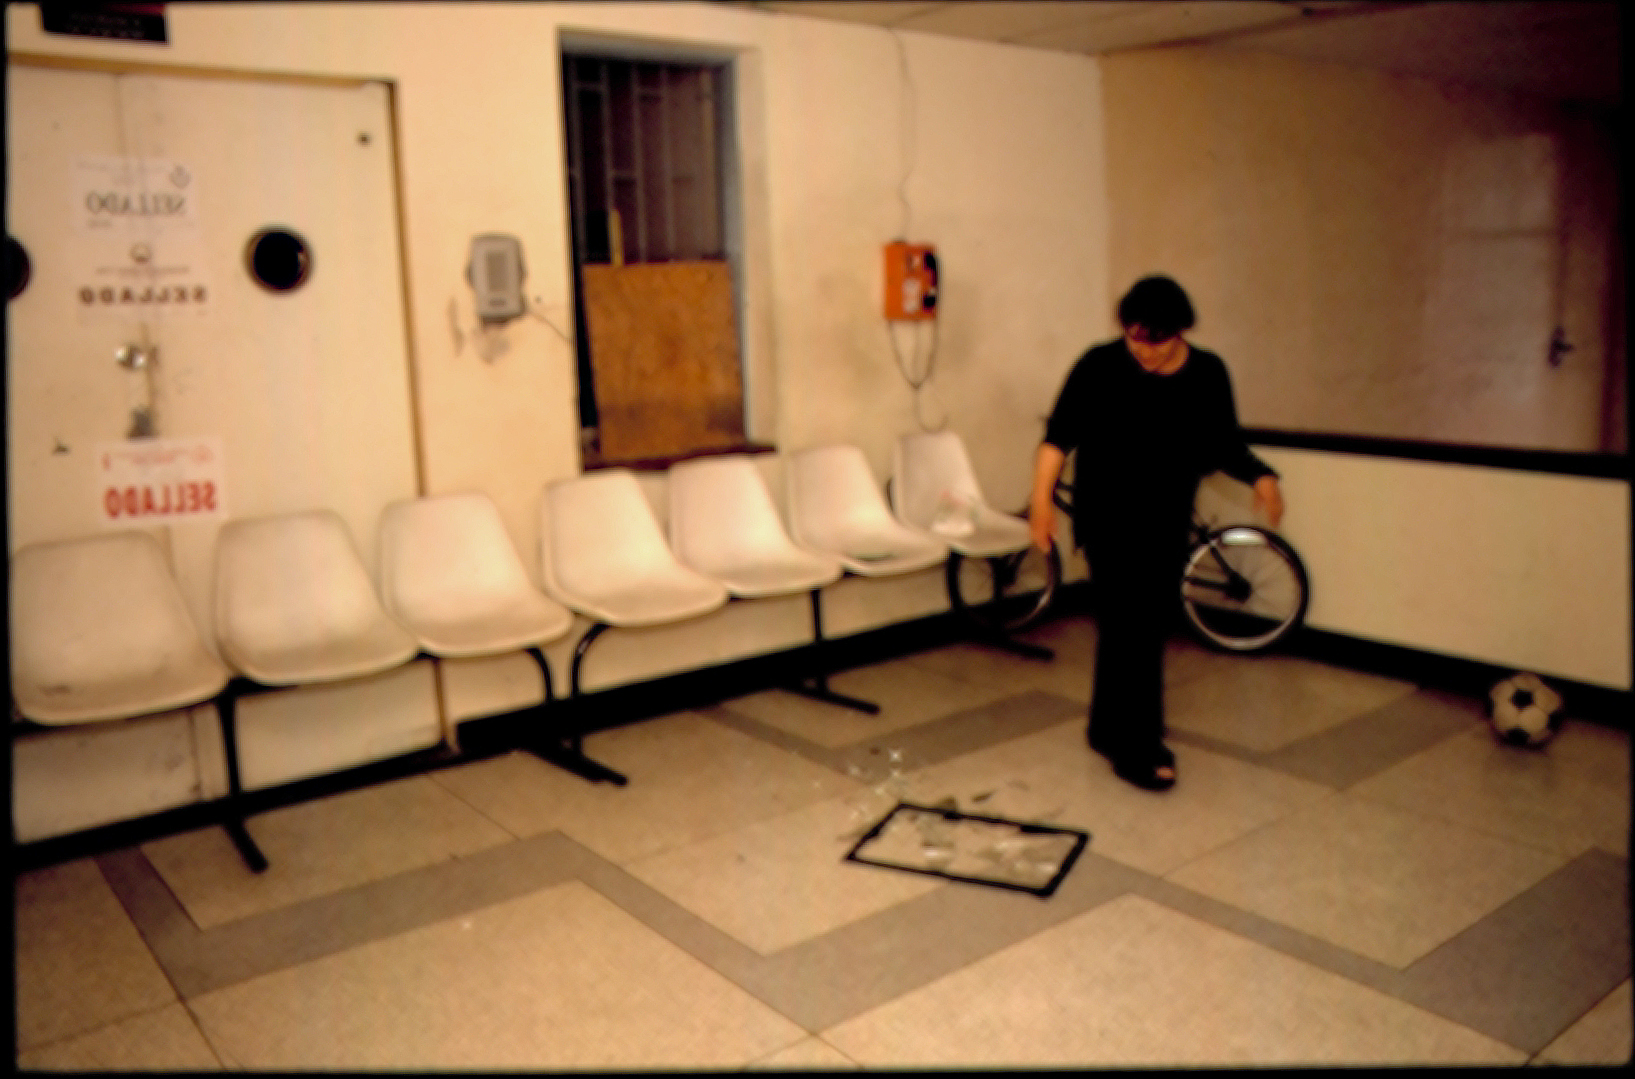
\includegraphics[width=\textwidth]{archivoMargarita_6octubre2004.jpg}
    \caption{Archivo Margarita 6 de octubre 2004}
    \label{fig:archivoMargarita_6octubre2004}
\end{figure}

Sala de espera con una fila de asientos blancos de plástico montados sobre una estructura metálica negra. La pared es de color crema claro con algunos elementos montados como un tablero y un teléfono naranja. El piso tiene un patrón geométrico en tonos beige y gris. En la escena hay una persona vestida de negro que mira hacia el suelo a lo que perece ser un marco y cristal rotos. Hay una bicicleta, un balón de fútbol y detrás de la hilera de sillas a la izquierda una puerta con letreros de `SELLADO'.

\small
\begin{verbatim}
graph TD
    A[[Anacronismo]]
    B[[Imagen-Síntoma]]
    
    A --> A1[Sala de espera vacía y austera]
    A --> A2[En tonos apagados]
    B --> A3[Lo lúdico se asoma]
    
    B --> B1[Soledad y aislamiento del individuo]
    B --> B2[Deshumanización en espacios institucionales]
\end{verbatim}
\normalsize

\clearpage
\begin{figure}[h!]
    \centering
    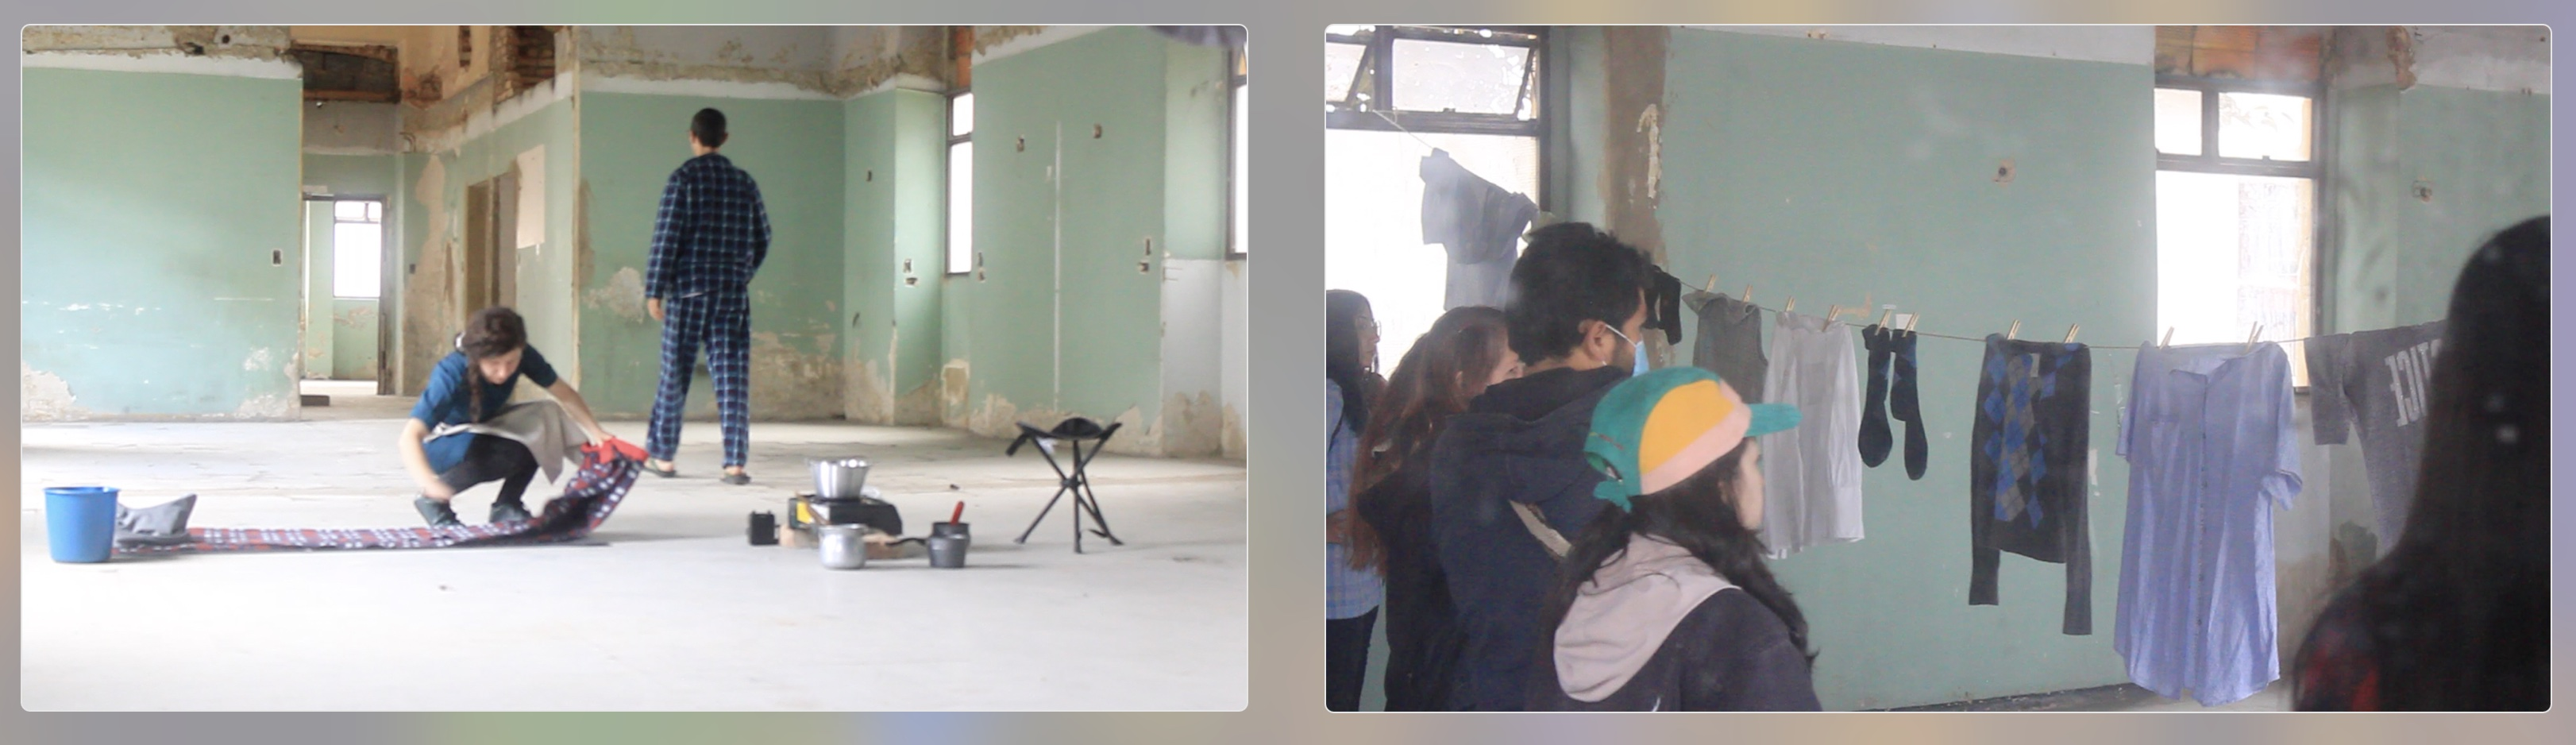
\includegraphics[width=\textwidth]{archivoJuanArroyo_10September2022_04_33.jpg}
    \caption{Archivo Juan Arroyo 10 de Septiembre 2022}
    \label{fig:archivoJuanArroyo_10September2022_04_33}
\end{figure}

\textit{Performance}. La imagen muestra edificio San Lucas en proceso de renovación o reparación. En la primera fotografía, se observan dos personas realizando tareas en el espacio - una sentada en el suelo trabajando con herramientas, y otra de pie observando. La segunda fotografía muestra a una persona sola de espaldas en el mismo espacio, se aprecia ropa colgada en una cuerda, dando la impresión de un espacio doméstico improvisado. Las paredes desgastadas, ventanas en crudo y suelo de concreto sugieren que el edificio está en una fase inacabada o de transición. Se yuxtaponen  escenas cotidianas de trabajo y vida dentro del entorno hospitalario.

\small
\begin{verbatim}
graph TD
    A[[Anacronismo]]
    B[[Imagen-síntoma]]

    A --> A1[San Lucas cambia]
    A --> A2[Ropa al viento susurra]
    A --> A3[Hogar casual]

    B --> B1[Personas habitando en contexto disruptivo]
    B --> B2[Ningún mobiliario]
\end{verbatim}
\normalsize

\clearpage
\begin{figure}[h!]
    \centering
    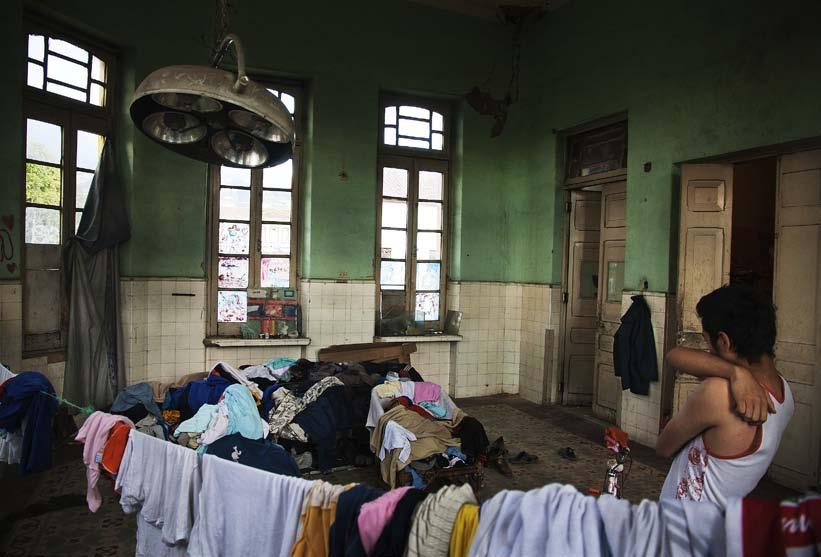
\includegraphics[width=\textwidth]{2011 Nicolas Van Hemelryck - San Juan sin Dios055.jpg}
    \caption{2011 Nicolas Van Hemelryck - San Juan sin Dios - 055}
    \label{fig:2011NicolasVanHemelryckSanJuansinDios-055}
\end{figure}

Sala de cirugía, interior deteriorado, ventanales que dejan entrar luz natural, contrastando con lámparas eléctricas colgantes. En este espacio se observan personas sentados en el piso sobre colchonetas y frazadas, rodeados de ropa y objetos personales. La escena revela síntomas de de usos disruptivos de ambiente para el cuidado quirúrjico y en hábitat doméstico. Foto del libro \parencite{Hemelryck2011}

\small
\begin{verbatim}
    graph TD
    A[[Anacronismo]]
    B[[Imagen-Síntoma]]

    A --> A1[Ventanas de otra era iluminan penumbras del presente]
    A --> A2[Despojos textiles de tiempos mezclados yacen inertes]
    A --> A3[Sombras del pasado acechan en la quietud actual]

    B --> B1[Abandono y precariedad se cuelan por los muros]
    B --> B2[Niñez expectante aguarda en silencio un futuro incierto]

\end{verbatim}
\normalsize


\clearpage
\begin{figure}[h!]
    \centering
    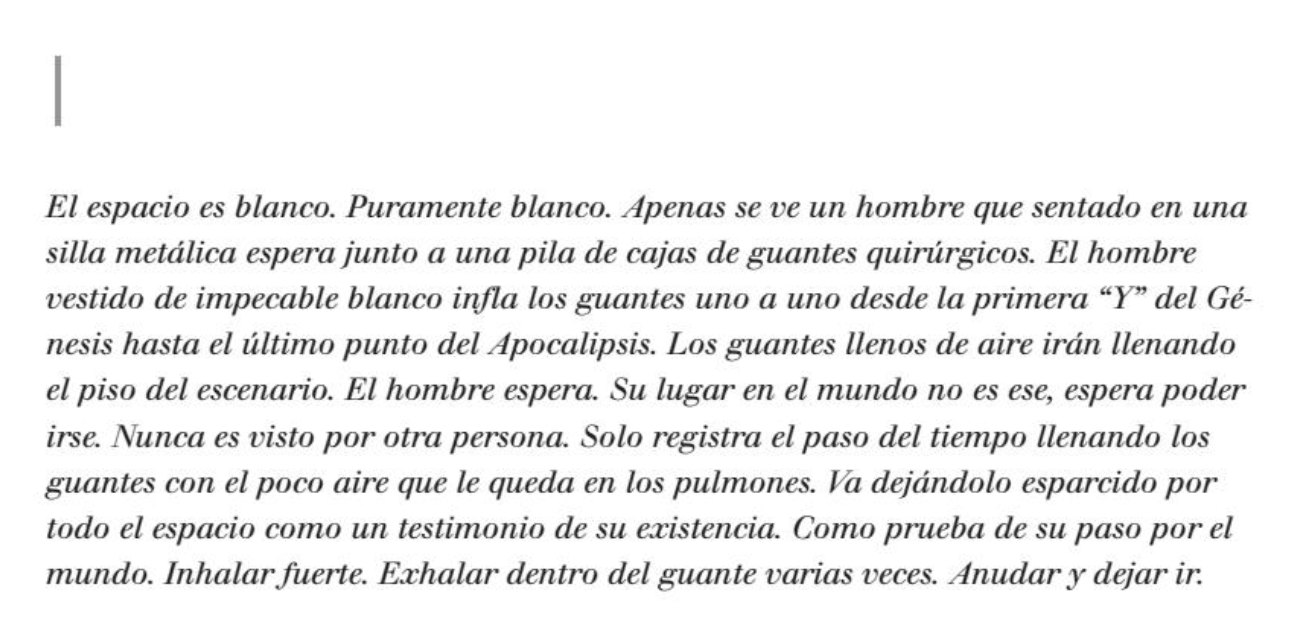
\includegraphics[width=\textwidth]{Ahumada2013_cuadro1.png}
    \caption{Cuadro I. Juan Camilo Ahumada, Tiempo de dios. 2013}
    \label{fig:Ahumada2013_cuadro1}
\end{figure}

\parencite[p. 10]{Ahumada2013}

\small
\begin{verbatim}
graph TD
    A[[Anacronismo]]
    B[[Imagen-Síntoma]]
    
    A --> A1[Impecabilidad atemporal y vacío]
    A --> A2[Guantes quirúrgicos y el aliento]

    B --> B1[Desconexión y falta de propósito]
    B --> B2[Automatización existencial]

\end{verbatim}
\normalsize

\clearpage
\begin{figure}[h!]
    \centering
    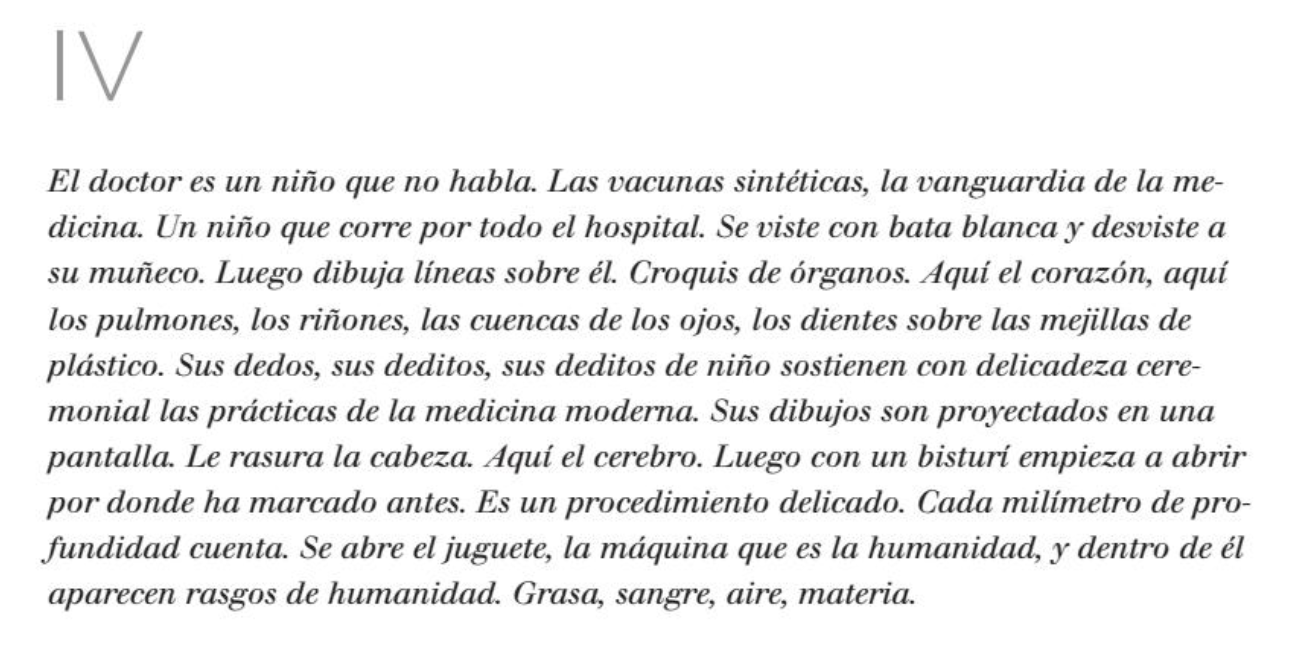
\includegraphics[width=\textwidth]{Ahumada2013_cuadro4.png}
    \caption{Cuadro IV. Juan Camilo Ahumada, Tiempo de dios. 2013}
    \label{fig:Ahumada2013_cuadro4}
\end{figure}

\parencite[p. 12]{Ahumada2013}

\small
\begin{verbatim}
    graph TD
    A[[Anacronismo]]
    B[[Imagen-Síntoma]]
    
    A --> A1[El doctor, un niño que no habla, cirugía moderna]
    A --> A2[Bata blanca y tecnología]
    A --> A3[La humanidad interna revelada]
    
    B --> B1[Avances médicos y fragilidad del cuerpo]
    B --> B2[Ética y cuidado humano]

\end{verbatim}
\normalsize


\clearpage
\begin{figure}[h!]
    \centering
    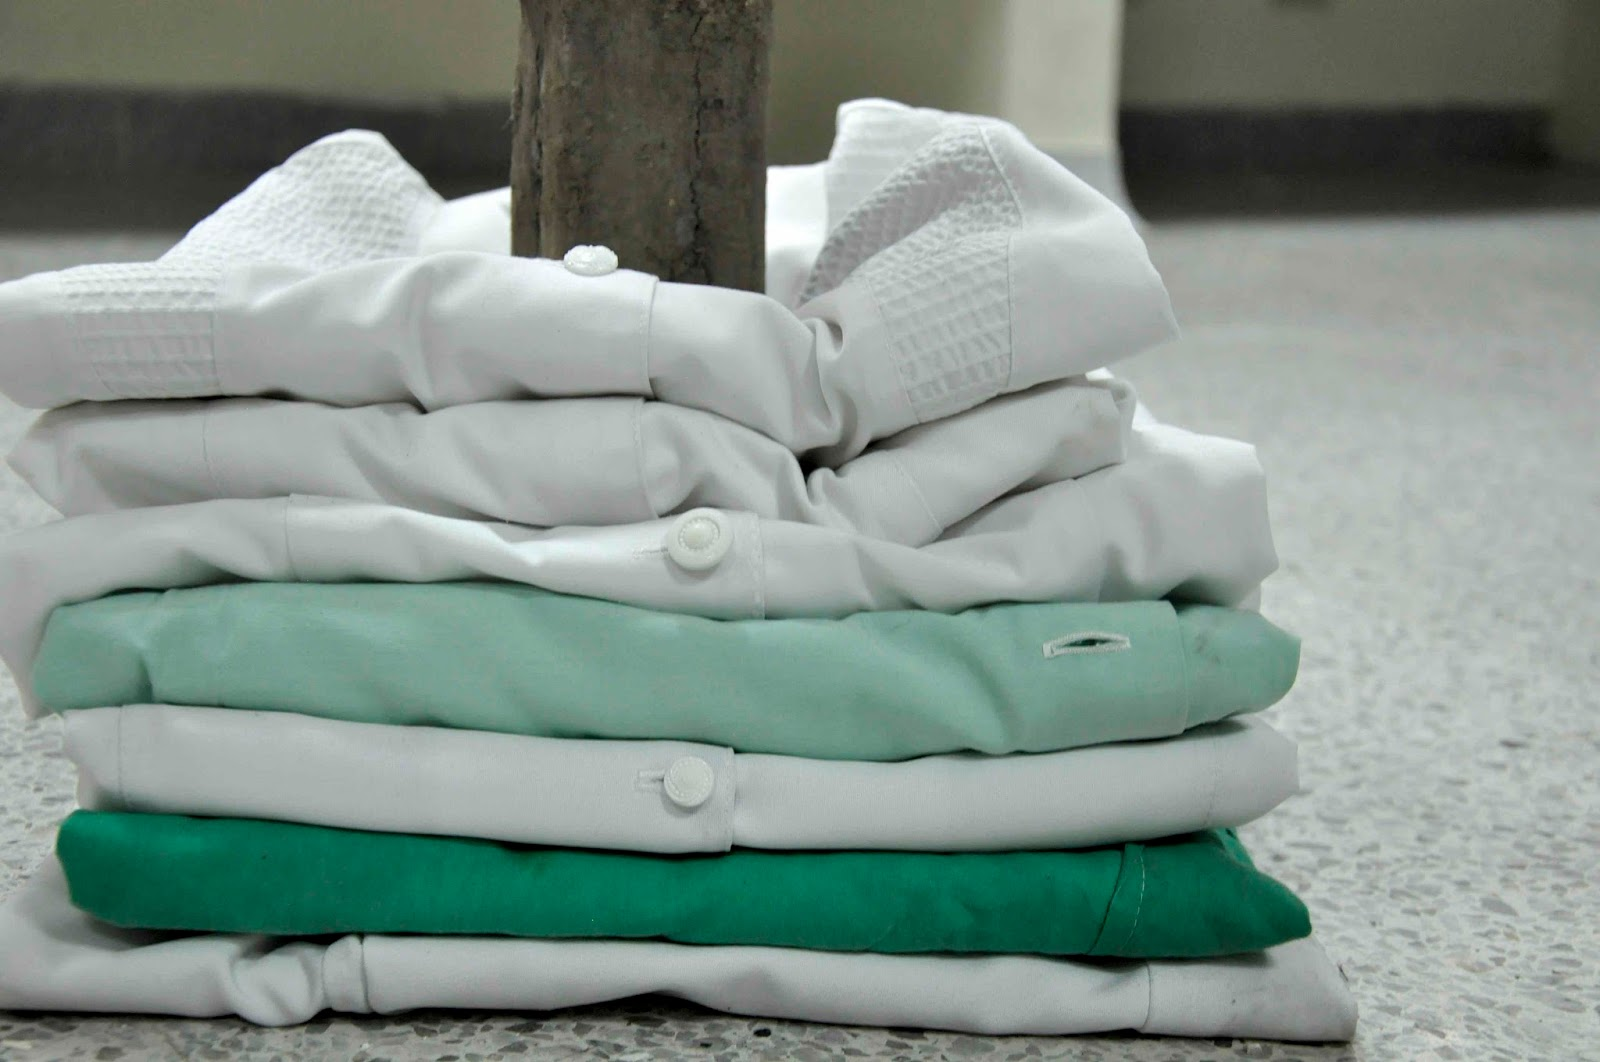
\includegraphics[width=\textwidth]{Una de las resistencias Karina Moreno 2015_5.jpg}
    \caption{\textit{Una de las resistencias} Ana Karina Moreno, 2015.}
    \label{fig:KarinaMoreno2015}
\end{figure}

Interior de edificio, postes de madera sosteniendo el techo sobre batas blancas y verdes apiladas. La tela se ve usada y pulcra, con arrugas y pliegues naturales.

\small
\begin{verbatim}
    graph TD
    A[[Anacronismo]]
    B[[Imagen-Síntoma]]
    
    A --> A1[Anhelo atemporal de pureza ]
    A --> A2[Contraste tela y rudeza natural]
    A --> A3[Ropa y pilar]

    B --> B1[Resistencia y fragilidad]

\end{verbatim}
\normalsize


\clearpage
\begin{figure}[h!]
    \centering
    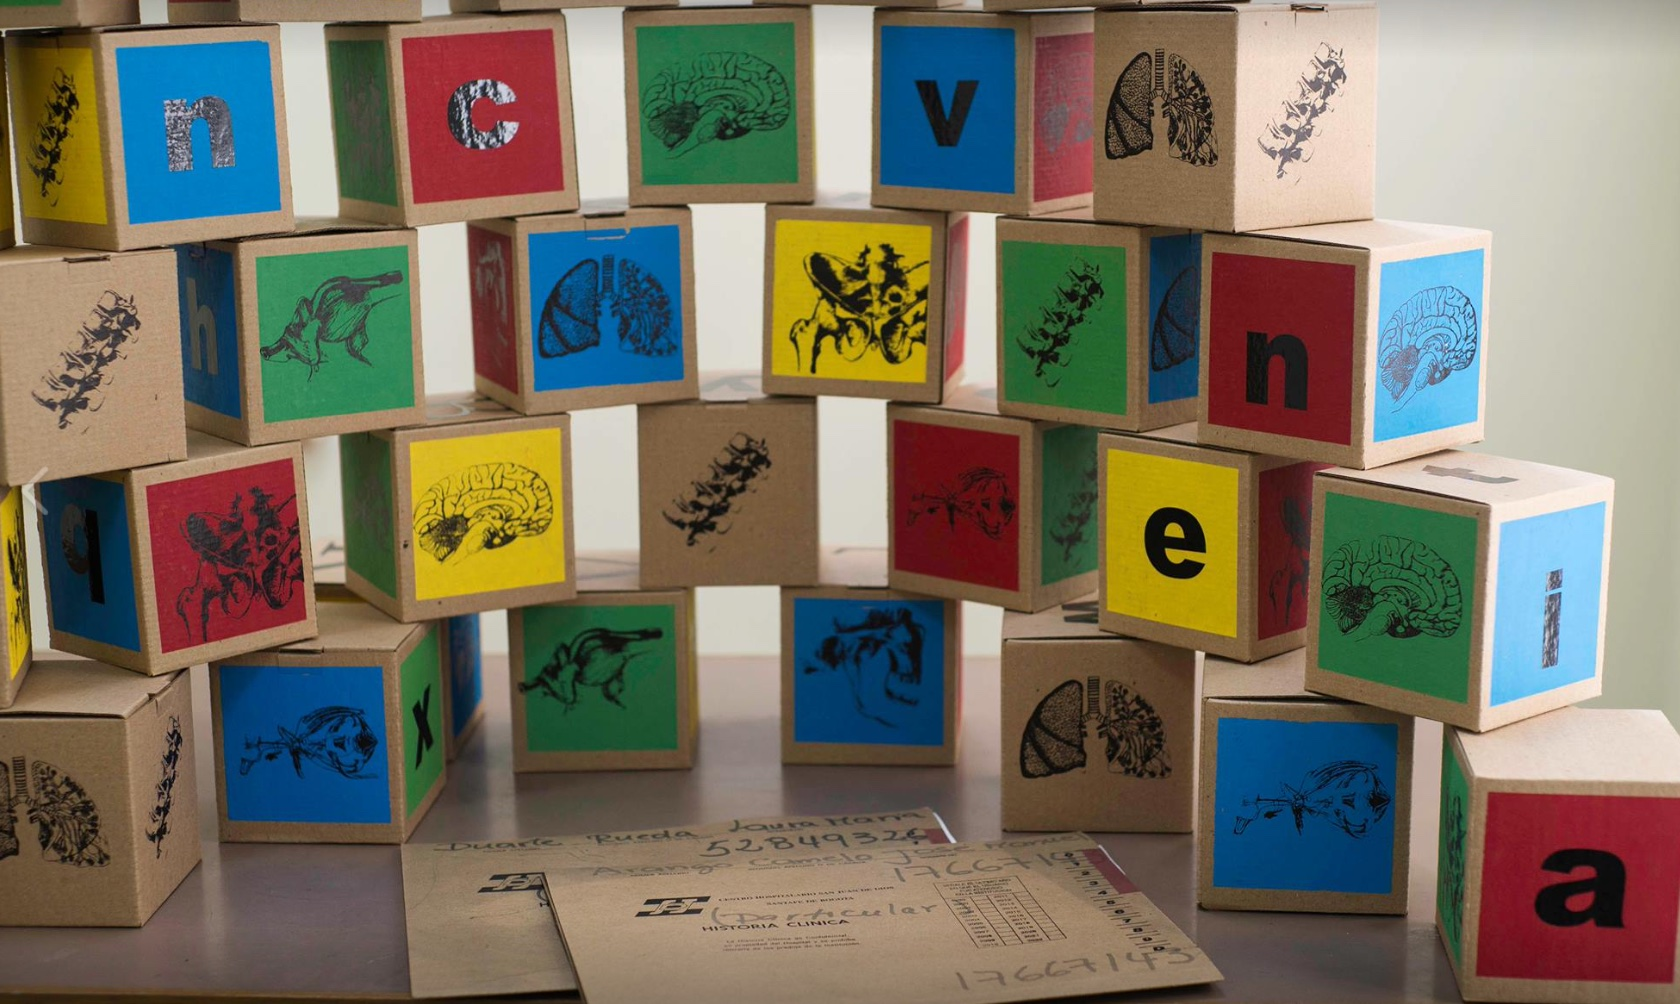
\includegraphics[width=\textwidth]{Duarte_didacticos.jpg}
    \caption{Didácticos para una sala de espera, Jenniffer Duarte 2015}
    \label{fig:JennifferDuarte2015}
\end{figure}

Colección de cubos apilados de madera, cada uno pintado con una letra del alfabeto y una ilustración en blanco y negro de diversos animales y partes del cuerpo humano, como cerebros y pulmones, en un estilo gráfico similar a grabados médicos antiguos. Sobres con hojas de historia clínica.

\small
\begin{verbatim}
    graph TD
    A[[Anacronismo]]
    B[[Imagen-Síntoma]]

    A --> A1[Bloques de juguete y grabados de ciencia]
    A --> A2[Lúdico infantil y la anatomía clásica]
    A --> A3[Fascinación perenne por el cuerpo]

    B --> B1[Alfabetización visual y biología humana]
    B --> B2[Curiosidad y asombro]
\end{verbatim}
\normalsize

\clearpage
\begin{figure}[h!]
    \centering
    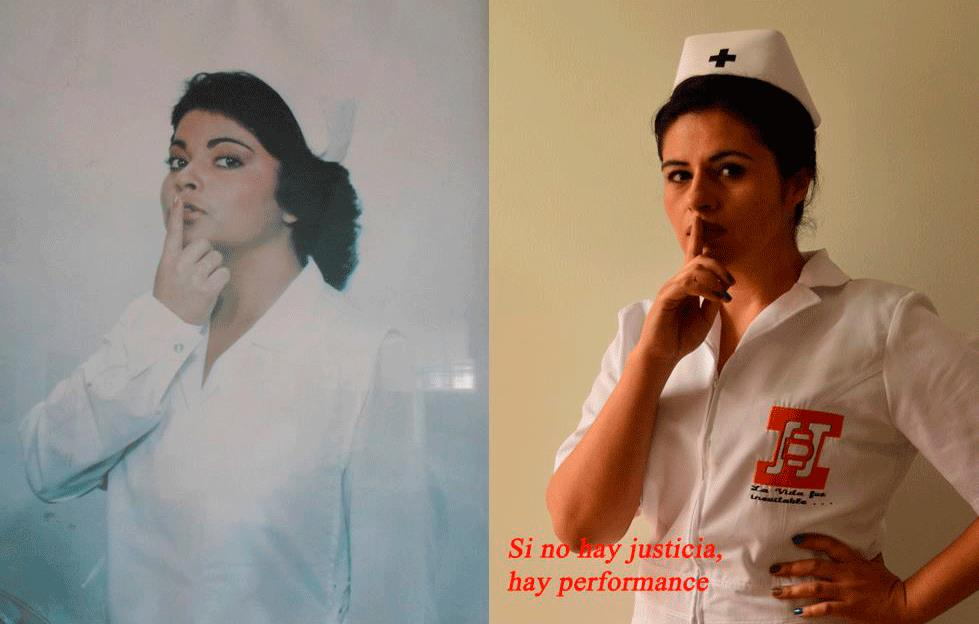
\includegraphics[width=\textwidth]{si no hay justicia hay performance.jpg}
    \caption{2016 Luisa Fernanda Vela - Al margen}
    \label{fig:LuisaVela2016}
\end{figure}

El montaje fotográfico yuxtapone dos retratos en blanco y negro de mujeres jóvenes de épocas distintas. A la izquierda, una imagen antigua muestra una mujer con peinado y ropa de los años 50, mirando pensativa con un dedo en los labios. A la derecha, una imagen contemporánea presenta una mujer con uniforme de enfermera y gesto serio, con la mano en la barbilla en actitud reflexiva. Debajo, un texto en español conecta ambas imágenes: ``Si no hay justicia, hay performance''.

\small
\begin{verbatim}
    graph TD
    A[[Anacronismo]]
    B[[Imagen-Síntoma]]

    A --> A1[Moda y peinados de distintas décadas se encuentran]
    A --> A2[Actitud contemplativa perdura a través del tiempo]
    A --> A3[Anhelo de justicia late en poses de mujeres pensativas]

    B --> B1[Mujeres en roles tradicionales cuestionan su realidad]
    B --> B2[Gesto meditativo surge ante injusticias presentes]
\end{verbatim}
\normalsize

\chapter{Escenificación: montaje de imágenes}
\vspace{4cm}
        
Espacio para las escenas 



\clearpage
\section{Conclusiones}

El montaje permite escenificar la emergencia de temporalidades, enunciaciones, anacronismos y otros síntomas en el conjunto de registros artísticos, imágenes documentales y textos visuales. A través de este proceso, se revela el entramado de atemporalidades y se genera una experiencia de sentido mediante los pasajes simbólicos del caso de estudio. El montaje constituye, entonces, un análisis interpretativo sobre la selección de imágenes que expresa espacial y temporalmente en <<cuadros>> el entramado visual y social, creando un ambiente de interpretación exploratoria que deriva en experiencias de construcción de sentido.

Denominamos escenificación tanto a la experiencia como al resultado del montaje utilizando las imágenes seleccionadas. El ordenamiento de las escenas representa una forma espacial de montaje que permite unir lo comprensible con lo imaginario, generando experiencias de sentido que confrontan nuestra mirada con el entramado sistémico de esta compleja situación social.

Las escenas materializan la intersección conceptual entre la antropología de la imagen y el método socio semiótico. La experiencia de inmersión en el recorrido visual sobre el San Juan de Dios ofrece posibilidades interpretativas que impulsan el deseo de comprensión, guiando al observador hacia la revelación de los entramados emergentes en este discurso no textual. Se omite deliberadamente el enfoque historicista, pues el objetivo es resaltar la existencia del anacronismo sin necesidad de una enunciación secuencial de acontecimientos.

El fenómeno sociocomunicativo del caso de estudio se manifiesta a través de elementos anacrónicos que atraviesan la imagen no-domesticada - aquella que se desprende de propósitos publicitarios o periodísticos - y se integra en redes dialógicas no-textuales mediante el montaje con otros discursos visuales. Esta interacción facilita la emergencia de la imagen-síntoma y los indicios de anacronismos.

La metodología propuesta permitió materializar objetos mediales para la conceptualización. El ``juego'' con las imágenes funcionó como estrategia de trabajo para abordar ideas abstractas, asociarlas y organizarlas espacialmente.

El montaje intencionado para la construcción de sentido enfatiza los síntomas visuales del discurso, generando conjuntos y redes significantes e imaginarias, interpretables desde los fundamentos conceptuales de la antropología de la imagen y la socio semiótica. Estas redes significantes o "fascinaciones" de la mirada subrayan la atracción irresistible del observador, quien en su gesto de registro o creación de imagen materializa enunciaciones emocionales y de sentido.

Un aspecto recurrente es el encuadre de lugares y objetos deteriorados por el tiempo: las imágenes evidencian el triunfo del agua, el musgo y la hierba sobre las superficies. Esta característica visible contrasta con el impulso de quienes han resistido y cuidado el San Juan, personas que han luchado a contracorriente mediante actos de expresión visualmente documentados, generando impulsos de resistencia ante la hostilidad del contexto y las circunstancias.


\addtocontents{toc}{\vskip10pt\hfill\textbf{|}\hfill\vskip10pt}

\clearpage
\listoffigures
\listoftables   

\phantomsection
\printbibliography[title={Bibliografía}, nottype=online]

\phantomsection
\printbibliography[title={Videografía}, type=online]

\addtocontents{toc}{\vskip10pt\hfill\textbf{|}\hfill\vskip10pt}

\footnotesize
\appendix
\chapter{Apéndice - Entrevista a Juan Camilo Ahumada}
\label{apendiceA}
Juan Camilo Ahumada
Juan Carlos Arroyo

Entonces te acabo de contar, sé que en el 2013 tu hiciste este… o por lo menos se publicó digamos.

Ahumada: Sí, eso.

Se publicó el guion, y en el 2016 hubo un performance, y en el marco digamos de esta exposición, el distrito hizo un evento con respecto a Arte y paz, y ahí digamos en el marco de esto David Lozano, que es un maestro en artes plásticas fue de la Nacho, hizo otro performance y entonces como que este es mi corpus de investigación.

Chévere, pues digo chévere estar como en la periferia de esas cosas, pues yo no… aunque trabajo en torno a los referentes concretos visuales, musicales pues de corte estético, y también unos referentes teóricos obviamente pues al afrontar como un ejercicio creativo, en este caso los referentes eran cosas muy, muy, muy distantes al hospital, porque era una cosa que era de alguna manera una premisa cuando yo arranqué, yo quería hacer algo a unos testimonios, primero vi la cosa es así. Me disculpa ser tan escueto, pero este es el proceso de creación, yo vi unos videos en YouTube sobre el hospital San Juan de Dios, obviamente como inquieto por hacer algo en torno al hospital San Juan de Dios y como tratando de indagar en quienes habitaban el lugar, porque lo que más me interesaba bajo este tiempo en el que estuvo cerrado, y algunas personas decidieron irse a vivir allá. La obra gira en torno a eso, básicamente entre lo que pasaba entre estas personas ahí adentro, e hicieron un intento de documental que colgaron en YouTube que está en acabado, estoy hablando como en el 2005 tal vez, finales del 2008 no se, por ahí antes del 2009 en todo caso.
Y luego me surgió la posibilidad de hacer una residencia artística en Buenos Aires, con un maestro de escritura gramática que se llama Alejandro Tantanian, y cuando yo llegué a Buenos Aires llevaba todos los materiales, todos los testimonios, y una suerte como de caprichos estéticos.

¿Y esos testimonios como los recogiste? 

Tenemos los del video.

a los del video ok.

Luego yo tuve la oportunidad de conocer una señora que se llama Teresa Díaz, que lideraba en ese momento, yo no sé ni siquiera si la señora está viva porque no tuvimos ninguna relación, nos vimos una vez charlamos y ya, yo la grabe en video. Y pues ella estaba como muy interesada en hablar como del movimiento político que se había ido gestando ahí, el ejercicio de resistencia civil y esas cosas, pero yo la sentía como decirlo, como muy en el terreno de lo político.

Si.

Yo quería cuestionar la cosa desde otros niveles. También porque a nivel de lo político eso estaba completamente sesgado entre buenos y malos, y los buenos son los que están ahí y los malos son los que los quieren sacar, como en la estrategia del caracol y no es así, la cosa pensarla de esa manera sería aplanar de alguna manera el conflicto, yo sentía que ya estaba aplanando el problema definiéndolos entre buenos y malos, pero de ella pude coger como una suerte de voz, y una suerte de melancolía en el ejercicio de habitar este lugar y todo esto se articulaba a la perfección como con una cosa que yo quería tratar de materializar que era como unos universos de la desesperanza, y en ese momento este texto surge con otros dos, es decir como en el mismo momento y por la misma inquietud con otros dos que son absolutamente diferentes, uno que se llama llenasvenbrandy y el otro texto que se llama noche de alacranes, que son también como unas obras que tratan de darle vuelta a esto de la des-absoluta esperanza, como de la condición humana en ese momento del ocaso de la vida, como de esperar la muerte, como que la única posibilidad de esperar sería esperar morirse y entretenerse durante la vida, como sin ningún oficio concreto bueno… y esta obra se ganó el premio distrital de dramaturgia y entonces logro como sacar la cabeza por ese trio de obras, pero igual las otras están ahí, llenasvenbrandy la montamos y era como de alguna manera la preocupación que tenía por la desesperanza, partiendo de la desesperanza llegaron los testimonios del San Juan de Dios, y hablándole a unos amigos de este proyecto que yo tenía, alguien me dijo que conocía quien dirigía el movimiento pues de las personas que habitaban allí, que era doña Teresa Díaz yo me reuní con ella, y con estos testimonios me fui yo quería también hacer algo entorno como a lo trágico, pensando en términos teatrales, es decir quería hacer algo que estructuralmente se pudiera definir dentro de lo que es la tragedia en el teatro. Y para eso entonces me apoye de una ópera que es este kindertoten líder, que son las canciones de los niños muertos, the mahler, había otro referente ahí bien importante que ahora no lo recuerdo. Bueno pero había otro referente de corte musical, y tratando un poco como de… esos son los insumos concretos digamos las materias con las que trabaje, ahora mi aporte pues gira en torno al tratar de construir dos universos ahí entramos hablar de la obra, yo creo que la obra se sostiene como en dos universos, uno que son las cosas que suceden al interior de las personas, como el terreno del pensamiento, de la evocación, o del recuerdo bueno en fin, las cosas que les pasan por dentro a las personas, y otro plano que se contrasta como de una manera medio abrupta también ahí en la obra es lo cotidiano, y de alguna manera es como lo ordinario, el orden normal de las cosas de alguna manera lo vulgar, lo escueto, trivial si se quiere la lógica de la cotidianidad de una manera más… es que la palabra no es costumbrismo, pero la cosa si es como de una forma mucho más concreta, las cosas concretas los panes, las mesas, los dados, las cosas concretas de la vida de estas personas, y en el texto trato de armar. Originalmente este texto puede que esto de luces, originalmente el texto se llamó viacrucis y era una idea de hacer las estaciones, la idea digamos como estaba pensado era como unas estaciones en el espacio y que los espectadores pudieran transitar el espacio viendo estas situaciones instaladas en diferentes lugares, entonces hay una estructura narrativa que no es lineal y que se sostiene como en la construcción de estos pequeños universos que son casi que independientes. Y estructuralmente pues el recorrido quedo así como si arrancara, como una suerte de vocación, en la mitad está toda esta tensión con la cotidianidad, con el mundo concreto y terminamos como tratando de romper esta idea de la esperanza cristiana y del tiempo de Dios.
Ayer un muchacho en el bus, un ex drogadicto mencionaba el capítulo y el versículo de Ezequiel 3:3 que dice que los tiempos de Dios son perfectos y que todo tiene lugar y tiempo en el mundo de Dios y bueno estas cosas, que era de alguna manera como la justificación que ellos me daban o que yo sentía de ellos y es que el tiempo de Dios es perfecto y esto va a durar lo que Dios quiera de alguna manera, porque también hay que decirlo esto sucedió antes del gobierno Petro, cuando premiaron esta obra que fue en la mitad del gobierno Petro el problema se estaba disolviendo es decir si ese texto no lo publican en ese momento pierde completa vigencia, aunque la relación ahí no ha sido asumida tan directamente digo como por la gente que lee y eso.

No pero tiene mucho sentido es decir por ejemplo para mí sería muy difícil no reconocer digamos el momento en que estas obras fueron publicadas.

Si tiene mucho que ver con eso, claro

Hay algo de mis hipótesis pero tiene que ver con que el discurso digamos político social encuentra ahí un fenómeno en donde confluyen muchos de los discursos que de una manera a quienes estaban metidos en la problemática les servía el discurso político, se prestan mutuamente los intereses.

Si como un terreno fértil no.

Si.

Un terreno fértil como para que todos de ahí saquemos una buena cosecha seguramente fue así, porque también el momento en el que yo estaba en estas, estaba dándose esto con el gobierno Petro, como las discusiones, las conversaciones, la posibilidad de negociar el predio con la gobernación de Cundinamarca y esto, y un poco como se veía de lejos, porque yo pude ver además desde Buenos Aires como se veía de lejos la cosa, era pues si estamos abonando el terreno y ya luego todos, además todos incluso el gobernador de Cundinamarca que en ese momento era un hampón, todos sacaremos provecho.
Y ya el ejercicio literario pues fue un poco darme la pelea por lograr ser un poco coherente en la construcción de estos universos, y el texto está construido por unos hilos como narrativos que tratan de vincular los diferentes fenómenos. Pero si quiere hablemos de las escenas sí.

Por favor.

Ya hablando de eso de las escenas que cada una tiene un universo independiente, pues este primer cuadro que es solamente una acción, que este niño que está inflando unos guantes y está dejándolos pasar tenía un poco… se lo voy hablar desde la intención literaria de la teatral.
En lo literario yo quería como de alguna manera instaurar un tono para el texto, una manera de escritura, una textura para el texto de alguna manera como abriéndole la puerta al espectador hacia la manera en la que yo quería narrar la  historia, y creo que teatralmente espacialmente esto nos permitía como construir una metáfora del paso del tiempo, en ese momento una premisa era como una apertura hacia la eternidad, como hacia algo que no tuviera fin, bueno en fin, y esta figura del niño que va acompañando todas las historias o que las va atravesando pues de alguna manera era como presentar el anfitrión que va a ir con la gente haciendo el recorrido, pensándolo así digamos.

Si.

Este segundo cuadro que es el de Rosalía, es la presentación de este personaje, Rosalía es un personaje real que habitó con ellos en el hospital y que efectivamente la mandaron a habitar al edificio psiquiátrico, y que además es un personaje bellísimo, yo no tengo ningún vínculo personal con ninguno de ellos, pero si tuviera que tenerlo preferiría tenerlo con Rosalía, porque a pesar de que tiene una distorsión del pensamiento y que piensa de una manera paralela digamos a la convencional, me parece una mujer de una sensibilidad absolutamente particular y era la única digamos que estaba… voy a decirle el gesto y usted hace la interpretación, cultivaba y tenía animales dentro del lugar y se había dado una pela muy grande porque le respetaran el patiecito donde tenía sus matas y cultivaba, es decir no solamente matas sino cultivaba cosas y cuidaba unos animales pollos, perros bueno en fin, y ahí yo vi como un gesto más de empoderamiento como muchísimo más agresivo y eso le significó estar alejada de  los demás, de todos los demás que estaban habitando el Hospital, y además estaban en una pelea constante con todos muy fuerte. pero Rosalía también tenía un hijo, que es un hijo que luego se va a convertir aquí en el invalido un hijo con una discapacidad que yo nunca conocí, al que siempre me mencionaron y que siempre tuve ahí como en un ideal medio macabro de un muchacho quieto dentro de una pieza o dentro de un consultorio convertido en pieza, estático mirando una pared, contando ladrillos en una pared sin posibilidad de moverse ni de prender un televisor, ni de escuchar radio, ni de hacer nada en su vida más que ver y contar los ladrillos de una pared.
Bueno pero entonces aquí básicamente la presentación de este personaje, y tratar de ir instaurando el lugar, porque ella arranca como contando… describiendo quienes habitaban unos consultorios de consultas en un primer pasillo.

Este tercer cuadro es la presentación de Teresa Díaz, a quien le adjudicó el hijo de Rosalía, si es decir el hijo de la vida real de Rosalía yo se lo pongo a Teresa Díaz y la pongo como en un juego hay de amor y odio con el hijo en esta figura que tal vez está más adelante, hay una imagen en la que ella está afeitando al hijo acá, afeitar al hijo es cuidarlo, acariciarlo y también querer acabar con su vida que era un poco como esta cosa como tratar de construir esta imagen de la mamá que tiene que afeitar al niño inválido pero que en algún momento piensa jalar la cuchilla y dejar ahí, dejar ahí pues.
Esta es la presentación entonces de la enfermedad del muchacho, y aquí vuelve el niño y esta lógica como de la práctica científica y destacas en las que ellos fueron tan diestros de la… como de la  concreción de su oficio que tenía que ver con sangre, manipular carne, mover viseras, ajustar compresas llenas de sangre, botar restos de seres humanos estas cosas, aquí trataba de metaforizar por medio de un juego de un niño que es cirujano y que trata de abrir dentro de un muñeco y tratar partes y sacar partes dentro del muñeco mientras eso es amplificado en una proyección, de alguna manera quería que esto, la imagen que yo tenía era como de una cirugía que estaba sucediendo adentro y que se podía ver proyectada en el hospital como si quitaran partes digamos del espacio y adentro encontraron partes humanas, de alguna manera como una vuelta ahí a la imagen que era una imagen de referente con la que yo me había sido de un niño rompiendo un muñeco con un bisturí, trate de componer esa… además de esta imagen salió este niño que era vuelvo y digo el elemento que nos atravesaba como anfitrión, como se llama el Aqueronte que va con uno atravesando pues haciendo el recorrido como anfitrión.

Pero dices del hospital arquitectónicamente?

Si. Espacialmente, y además esto es una cosa que luego se volvió bien difícil, y es que yo escribí esto para ese espacio, pensando en ese espacio y nunca, nunca pude ni siquiera pensar en un proyecto creativo que tuviera que ver con eso y tuve que quedar satisfecho.

Pero recorriste ese lugar, digamos físicamente?

Sí, es decir está y hay una de las escenas que es esta donde están con el padre y que están haciendo como unas oraciones, está la del animero, es un recorrido por un espacio real y yo trato de darme la pela por describirlo, aunque pues es que yo soy muy mal autor entonces no lo logró describir a cabalidad, pero la idea si es que aquí quede el espacio todo esto del ritual del rezo y tal, aquí entre nos pues digamos es una manera de construir el espacio, y es una manera además densa y aburrida porque esto estructuralmente supone un momento que la obra pare como después de ir en quinta, mandar a primera de una y que toca haga como… y vuelva a instaurarse en otro ritmo muchísimo más lento.

Ya.

Que es un problema digamos para el ritmo de la obra, pero era necesario porque yo quería el recorrido espacial, es decir quería la gente en una procesión con esta lógica además del animero paisa que no se si conoce esta historia del animero, de un tipo que quería tal cual un poco como animero coro de actores haciendo de almas y espectadores transitando la representación.

Guiados por ese animero.

Si, si y construyendo el espacio a partir de eso, y había otro referente importante en esas tres obras además, yo creo que también un poco en mi manera de escribir y mi manera de articular las historias o de contarlas y es la cultura popular, obviamente distanciado del teatro popular y esas cosas que no tienen nada que ver con esto, pero si quería un poco tratar de también cuestionar esto desde la cultura popular, es decir esto como se pensaría también la nostalgia si el único referente posible fuera Alci Acosta.

Aja ok.

Si como ponerles palabras al dolor si el único referente es Vicente Fernández, por decirlo de alguna manera, o Roberto Carlos que aparece acá tratando de escribir una relación amorosa con un tipo que solamente escucha Roberto Carlos que es un personaje muy indo.
Y ahí empiezan aparecer este tipo de cosas, por ejemplo como esta escena es la escena número cinco de Edelmira, en la que hay como una suerte de rezo en la que ella está sola, en un espacio como con unas imágenes sagradas, y está tratando de construir como una suerte de rezo como de oración que se intervenía por este tipo de cosas que son los Visconti además, aquí juego como con las palabras de la oración y de la canción, el editor muy inteligentemente divide las cosas y  les pone negrilla a una cosa y a la otra y tal, como un poco para profundizar más en el guiño que fue un gesto que a mí me pareció muy bonito.

Empezamos hace un rato, en este momento Juan Camilo digamos me está contando a través de los cuadros, tanto la intención como un poco el gesto en el proceso de la creación.

Si, se fue digamos como materializando cada escena, yo estaba diciendo que cada escena funciona de alguna manera de forma independiente, como un solo universo dentro de una lógica estructural que se propone como un recorrido.
Cada una de estas escenas significa un espacio y  significa como una línea de acción que se cierra a sí misma, es autónoma pensándolo en términos narrativos, que es autónoma, una historia que se cuenta completa digamos, no necesariamente una historia con conflicto y solución y estas cosas, pero es una historia autónoma completa. Luego acercándonos ya a la mitad un poco de la pieza está este cuadro que es el del inválido que es el que yo creo que he logrado materializar de manera muy clara la intención inicial que yo tenía que era esta de poder ahondar lo que pasa por las cabezas de las personas que perdieron la esperanza por completo, estas personas que están un poco… yo decía ahora como en el ocaso de la vida bueno en fin, y este es un cuadro en el que se tratan de describir unas acciones, hay una contradicción pues planteada de entrada, y es que yo propongo un texto de cuatro páginas y digo que es un texto para ser bailado.

Ok.

Para ser bailado, para dar cuenta de la imposibilidad del  movimiento, y también un poco como insistiendo en esa incoherencia, pongo al muchacho sin palabras, el muchacho que no tiene acceso al lenguaje lo pongo a llenar de palabras, las sensaciones, estado en el que está, un momento muy específico en el que él está mirando en el patio, está mirando una pared contando ladrillos y viendo bichos que se cuelan entre los ladrillos, tratando de dar cuenta de la inmovilidad desde unas contradicciones, como tratar de contradecirlo para evocar esta inmovilidad, y obviamente también hay como unos gestos ahí, como unos guiños con estas cosas por ejemplo como de denominar lo inválido y no ponerle otro nombre con toda la fuerza y la agresividad además que tiene esa definición, invalidar deberás o anularlo lo que no vale, la silla, la silla que se pueda acomodar, y también pues esto responde a mi interpretación de esa relación de la mamá y del hijo, del hijo que ni siquiera decidió irse a vivir ahí, sino que fue porque tenía que estar con su mamá.
Esta primera escena que es del otro plano.


Si, a mi me llama… mientras la pausa para que no se me escape un poco lo que… y es que digamos te contaba un poquito en el correo cuando hablamos por el correo no, por el chat te contaba que digamos para mí esta pieza frente a todas las del corpus que estoy investigando es la que digamos me causa dificultad, pero ahora que te escucho empiezo a encontrar unas cosas, y es que finalmente yo me paro a hacer digamos un estudio sobre la imagen. 
Entonces cuando yo la leí digamos que evidentemente para mi tanto por cómo lo estás narrando y como información digamos como artista plástico digamos que yo me pinto el cuadro no, empiezo a leer y yo me pinto el cuadro. Ahora tal como lo cuentas encuentro que si efectivamente hay digamos una intención fuerte de construir una imagen de un momento específico.

Sí, y también de alguna manera yo pensaba el texto como un indicio sabe, que es una cosa bien distinta a los otros ejercicios de escritura, y es que esto pretende ser como un indicio, una pista sobre cómo construir espacialmente la obra, porque si creo que la cosa se escapa de la narrativa convencional teatral, sí es decir el teatro casi que se podría definir por la acción dramática, por lo que hacen los personajes, en este caso de alguna manera la obra si está planteada como un cuadro vivo digamos, en estos cuadros vivos de los católicos que es un cuadro con pequeñas acciones que no tienen mucho desarrollo, que es una cosa muy pequeña, pero que queda un planteamiento absoluto, absolutamente claro casi que de una época, de unos personajes, de una relación y de un espacio específico.

Son acciones que tienden a ser repetitivas, en esos cuadros vivos…

Si.

Casi ellos lo que construyen corporalmente es un ciclo, repiten un movimiento.

Eso es, y en esta lógica además del recorrido era un poco como yo pensaba el trabajo de los actores para asumir esto, y era de manera cíclica, es decir que una escena pueda terminar con el comienzo de esa misma escena, y esta escena que estamos… que vamos hablar creo que da cuenta de eso, perdón no es esta es la segunda de este mismo universo, que es esta con la que empieza con los tipos que están jugando dados, cuatro tipos uno que se encargó de oficios generales, el otro del transporte bueno en fin, que están jugando dados y la escena empieza con esto de anoche llamó el abogado que dice, seguro que esta semana sí, que eso está de un pelo, así empieza la escena le dan toda la vuelta, que la vuelta también es como en medio espiral, para terminar con esto, anoche llamó el abogado que dice, seguro que esta semana sí, que eso está de un pelo, más o menos, malparidos tal cual como empezó, tal cual, como dejando claro que es que la lógica si es circular, como no hay desarrollo, y eso va un poco en contra de la manera de escribir más teatral que necesitaría un desarrollo, y que sus acciones lleven a algo, que se articulen dentro de la noción de progresión dramática ya que esa progresión no existe, porque quería era que ahondáramos en ese universo de esa pieza de estos hombres que trato de escribirlos además como con detalle visualmente, cómo están vestidos, con que materiales, bueno en fin.
Y bueno pues estas dos escenas plantean dos cosas, como dos fenómenos que a mí me parecían necesario mencionar, y uno tiene que ver con el hambre y lo que pasa con la comida en estas situaciones, y la comida como la cosa más ordinaria, vulgar, cotidiana, concreta, humana pues comer, y la importancia que tiene comer y tener comida y cómo esto se chocaba esta cosa sobre la comida y sobre la ausencia de comida del padre y de la hija, de la plata y bueno de esta cosa, se contrasta con la discusión familiar que supuso tomar la decisión de irse, por un lado y por otro lado la anécdota que también ustedes conocen sobre la ambulancia que llevaron al INPEC.

Si.

Que era una ambulancia que ellos utilizaban para ir a abastos, que ese es como el subtexto de esto porque eso no está aquí solamente decimos que se llevaron la ambulancia del INPEC y que son unos hijueputas, y que se la trataron llevar otras veces y tal, porque deberás hubo ahí todo un operativo para sacarles la ambulancia, según ellos lo cuentan, ellos tenían que hacer vigilancia y una vez que los emborracharon y los cansaron y tal, le sacaron después la ambulancia con la complicidad de los celadores que siempre estuvieron riñendo con ellos bueno en fin, entonces esta ambulancia era importante y que se la había llevado era importante yo lo vine a comprender mucho después, era porque en ella podían ir hasta abastos y en abastos les regalaban comida, por eso me parecía importante dejarlo en este momento estructural que les mencionaba yo ahorita, como es el de lo concreto, el de lo operativo de alguna manera, lo que hay que hacer para que esta cosa funcione, y pues una grita también que para ellos supuso una grieta en el movimiento y una cosa muy fuerte esta cosa de que les quitaron, les quitaron de alguna manera una conquista que han logrado que era también tomarse este marica carro que todavía serbia.
Luego viene este recorrido espacial el del animero que tiene que ver con esta cosa paisa yo decía que también además es como un fenómeno paisa muy amarrado a la violencia en Colombia, y a los fenómenos violentos en Colombia, esta cosa de ponerle nombres a las almas y a esto que paso también el Valle fue, Trujillo Valle.

No, no sé.

Un pueblo que se tomó unas víctimas, iban encontrando víctimas por el río, hom,bres y los fueron sepultando y les ponían nombre y después les iban pidiendo favores, después de estos favores, de que estos favores fueran concebidos les iban dando apellido, el de su familia y los iban metiendo de alguna manera a su familia les decoraban la tumba, las flores unos N.N completos, y esta comunidad también hacia esta práctica de animero de un día al año ir y sacar a las almas a darles una vuelta por el pueblo y devolverlas otra vez para el cementerio, y tratando de pensar en eso pues aparece esta escena que también aquí en esta obra nos permite poner al espectador  a pisar las baldosas, a ver el piso, a ver el color de las paredes del hospital un poco como sin ningún tipo de  tratamiento estético que era el planteamiento, era andar el espacio y dar cuenta también de esta esperanza tan cristiana pero yo decía, o esta interpretación tan cristiana de la esperanza de que el tiempo de Dios es perfecto y que vamos a estar aquí el tiempo que Dios quiera pues eso es además lo que le da el nombre a la pieza, esta cosa de Ezequiel 3:3 de que en el mundo de Dios todos tienen su tiempo y todo tiene un tiempo y que bueno yo no sé cómo es que es que diga exactamente, pero básicamente dice que Dios es quien decide el tiempo en el que suceden las cosas de los hombres…

Y es perfecto.

Y pues así funciona la cosa, que hay que callar y agachar la cabeza y pues entender eso como la posibilidad más esperanzadora que tienen, pues es bastante desesperanzador digamos.

Bien y aquí cuando aparece este cuadro de las voces, pues es un intento por articular dos cosas, lo primero es la presencia del radio, del radio y del sonido del radio en el hospital mientras estas personas habitaron, cuando yo tuve la oportunidad de conocer el hospital fue una de las cosas que más me impactó como el contraste del sonido de los radios, yo fui en una tarde y en la tarde había tres programas de radio distintos en diferentes lugares, pero cada uno tenía su radio y su voz acompañándolo y nadie estaba pendiente de eso digamos era como un sonido de fondo en el hospital de alguna manera, yo quería materializarlo con unas voces que estaban dentro del hospital, unos tipos que estaban emitiendo el programa de radio, y el programa de radio es básicamente una descripción de diferentes fenómenos, este primero hombres rajados por la selva tal, masacre de las bananeras primer momento, masacre de las bananeras y esto tiene que ver también con el origen del hospital y la trayectoria del hospital quería dar cuenta por este programa de radio por todos los momentos de la historia nacional que el hospital de alguna manera testiguo, lo protagonizó algunos casos.

Si.

Entonces paso ahí por la masacre de las bananeras, más adelante el Bogotazo y Gaitán, la violencia y la lucha liberal conservadora y todo el fenómeno de la violencia posterior al Bogotazo, luego la toma del palacio de justicia y luego el narcotráfico, donde está la cosa sobre el narcotráfico, hay un momento en el que mencionan los aviones, que los aviones detengan su marcha pensando en ese atentado de los narcotraficantes al avión éste, y la explosión del avión y posterior la toma del palacio de justicia, a bueno y terminamos con esta cosa del narcotráfico de los precios, de cuánto vale todo, de que todo tiene un precio, de que pongámosle precio a todas las cosas.
Y bueno nos quedamos en eso de la violencia de los cincuenta, con esto que también son guiños a estos teóricos que yo mencionaba	 al comienzo, y casi que teóricos cliché de la violencia en Colombia por decirlo de alguna manera, muy chambona pero por decirlo de alguna manera como María Victoria Uribe por ejemplo, tú tienes el texto que se llama matar rematar y contramatar en el que describe los cortes, los cortes específicos y los mecanismos específicos de cada uno de los bandos durante el estado de violencia bipartidista, entonces por eso esta cosa de que quiero tener la cabeza entre las piernas, quiero tener un corte de franela, quiero que saquen mi lengua y que la cuelguen como una corbata, es un poco como unos guiños a esta manera a esta mujer de describir la violencia a partir de los mecanismos, y si al final cerramos pues con paramilitarismo y masacres paramilitares con esto que era también una preocupación muy grande en ese momento que trata de materializar llenasvenbrandi que es la masacre del Salado, como tratar de entender cómo funcionó de alguna manera la masacre del Salado, era otra cosa que me preocupaba en ese momento como una escritura paralela que estaba haciendo a esto, por eso también aparecen estas figuras que pues la imagen trata de definir un poco la masacre del Salado, los vi llegar en enormes bestias, devorarnos, quitarnos los brazos y las piernas, los vi arrastrar mi cuerpo alado por caballos, los vi correr, hacer música con tamboras y gaitas mientras me desmembraban quiero respirar un minuto de silencio bueno, esto pues son imágenes que yo creo que todos quienes conocemos un poco de lo que paso pues tenemos en la cabeza y es esta cosa de la mujer jalada por caballos y destrozándose su cuerpo por todo el pueblo, los hombres jugando futbol.

Y la música de…

Y la música… y estos tipos que van y se meten a la iglesia que sacan las gaitas y los tambores mamados de los gritos, borrachos empelucados empiezan hacer música mientras degollan o juegan futbol con cada vez...buen en fin.
Y esto ya para ir cerrando que es el cuadro de Rodríguez que es volver otra vez a ese universo de lo poético y vamos como más…

Mental.

De lo mental, de las evocaciones, y es presentar de alguna manera este personaje en esa misma tensión como por buscar que la cultura popular logre definir lo que este tipo siente, entonces este tipo se llama Rade Roberto Carlos que es lo que más ha querido en su vida y que el además se cree cantante que canta como Roberto Carlos Y bueno en fin, y muestra un cuadro que tiene un tono bien costumbrista, bien cotidiano, muy tranquilo, pero que muestra también un personaje que navega pues, como que circula, que bucea como en cierta ignorancia y  que trata de interpretar el mundo desde su ignorancia y desde su… voy a… si es que soy muy grosero con el lenguaje pero… desde su miserable manera de ver las cosas él trata de mencionar como los momentos en los que se ha sentido más pleno, más lleno de vida, y pues eso tiene que ver con el amor y con la construcción afectiva que pudo construir, hacer con una mujer, y como esa utopía alcanzada se vio rota en el momento en el que él tuvo que decidir me voy para el hospital, y que la tuvo que dejar y ahí más nunca volvieron hablar y la cosa se rompió como tratando también de dejar una historia de amor inconclusa, tratar de dar cuenta un poco del vacío en el mar de la desesperanza, de la ausencia, porque él mismo dice si yo me le aparezco yo no sé ella con que me saldría a estas alturas del partido, y pensándolo también en términos del señor pues digo el señor de 60 años, de 65 años que todavía piensa en su mujer como su amor, pero que ya no sería capaz de presentársele porque sabe que probablemente esté con otro tipo y la cosa sería muy complicada y bueno en fin.

Aquí aparece el cuadro de amar que se amarra con ese, de la afeitada del hijo, y del conflicto Teresa y su hijo, Teresa contempla a su hijo con algo de desesperanza y su hijo la ve desvanecerse en medio de una nube de humo tratando como de concluir un poco como este gesto con el que ella inició, y aquí aparece esto the mahler que es una ópera muy trágica, que se llama canciones de los niños muertos y que básicamente es un poema que escribió un papá sus niños como a finales de 1800 se murieron de una enfermedad pulmonar, digamos tuberculosis, y el tipo compuso una serie de poemas todos terriblemente trágicos y dolorosos en término de lo que significó para el perder a sus hijos y perder con ellos la esperanza de ser alguien, porque él había dejado toda su vida por sus hijos y a sus hijos se los llevó un virus, este cuadro trata un poco de dar cuenta esa misma sensación pero puesta en Teresa y viendo la imposibilidad de dar un otro estado a su hijo, de producir otra cosa, otra vida para su hijo y de ver acabada pues su esperanza que se debería materializar por medio de él verla rota.

Bueno, Edelmira y volvemos a Edelmira que es este personaje del lío mental que mencione antes, tratando un poco Edelmira de continuar en esta misma lógica que es la lógica del inicio, de cerrar de manera circular de cerrar su círculo, y ella cierra su círculo siendo en caso de que llegue a solucionarse la cosa ella lo que más esperaría de la vida sería irse para ese apartamento un poco como esto, desde aquí alcanzo a ver ese apartamento y me he emocionado tanto con él, que en caso de que yo me llegué a ir de aquí yo quisiera irme a vivir allá, que es un poco como dar cuenta de la imposibilidad y del poco mundo que había ahí que es ella mirando desde las terrazas del hospital hacia el Policarpa o hacia el samber es decir o una olla o un barrio proletario de donde venden telas, obviamente el barrio de telas es un lujaso pues un lujaso comparado en el momento en el que estoy y con la otra posibilidad que tengo, esta era el mundo de alguna manera que ella podía asimilar y yo trato de cerrar... 

El mundo al alcance de sus ojos.

Claro, con ella diciendo eso que el mundo llega hasta donde yo miro como en el feudalismo medieval, el mundo va hasta ahí hasta donde me alcance el ojo, y este cuadro también pues obviamente tiene la intención de cerrar la intención pesimista de cerrar en ese mismo plano pues desesperanzador, desalentador de encontrar a un en la esperanza de estas personas pues como una misión muy miserable por decirlo así, una ilusión muy mínima, muy escasa.

Ella trata de comparar eso además con la casona con la que vivió con su papá que fue magistrado, que tuvo otro estado, con el que tuvo otro tipo de vida en el que fue muy feliz, pero entendiendo la felicidad también como Rodríguez, entendiendo la felicidad como una cosa distante, ajena, perdida en el pasado de alguna manera y pues cerramos con este pequeño monólogo que es femenino el texto no dice más, es como un gesto del autor para cerrar es un gesto mío que intenta cerrar con voces femeninas o con una voz femenina describiendo este texto yo lo voy a leer.

Anoche soñé con olas, he empezado a mortificarme por lo que fue, por lo que pudo haber sido y no fue, eso es como la premisa para todo este texto, me lamento hasta en sueños no conozco el mar, supongo que alguien debe sufrir por una razón más justa, más profunda pero yo no, es la idea como de poner al personaje a mirar su esperanza, verla rota, reconocer y entender que su esperanza era mínima y la fractura que supone ver esa esperanza diluirse pues tampoco puede ser tan grande pero es su sufrimiento mayor, y era su ilusión mayor de alguna manera, y quería también ponerlo como en unos términos muy sensibles pero también muy aterrizado a la tierra, es decir cómo ponerla realmente a lamentarse por una cosa que es muy distante a nosotros los Bogotanos, que ha sido distante a demás tradicionalmente esta cosa de la tierra caliente y el mar, todo lo que significa para nosotros el mar, para nosotros que estamos tan lejos y lo evocamos pues, y que hablamos de él  todo el tiempo.

Siempre es importante, la primera ida al mar del rolo es importante.

Claro que sí, y esta sensación de las piedritas que se mueven por debajo de los pies ya que tocas eso, pues tiene que ver con mi primera sensación al mar, que yo recuerdo pues iba en una lancha para un lugar cerca de Acandí y me baje de la lancha ya en el momento en que se bajaron a dejar unos bultos y lo primero que sentí fue que el agua se llevaba las piedras debajo de mí y que yo me iba a hundir, esa sensación era como mi zumo para hacer esto, hoy mi dolor es solo ese, y bueno aquí entre nos tengo que confesarles que como recurso mío, propio para este texto pues estaba pensando en mi mamá, como pensaría mi mamá el mar porque siempre me impresionó mucho cuando yo crecí también cuando conocí el mar por cosas de trabajo y tal en fin, me empezó a preocupar de una manera muy rara que mi mamá no conociera el mar, como que hubiera alguien además cercano a mí que yo quisiera tanto tal, que no hubiera nunca tenido esa sensación, sin conocerla entonces la puse a ella a lamentarse por esa sensación que desconocía y a describirla con detalle, como esta de las piedritas. 

Me duele nunca haber escuchado el sonido de las olas golpear contra las rocas, o deslizarse llevándose la arena y dejando piedritas pequeñas desnudas en el suelo, que es una imagen bien precisa y la pongo igual a construirla desde la pura ignorancia de esta imagen, lamento no haber sido arrastrada por una fuerte marea hasta no sé dónde, nunca sentí las olas venir hasta mí y llevarse la arena bajo mis pies, nunca, me duelen las cosas que nunca me pasaron más que las que sí pasaron y quisiera olvidar, me duele aquí en el estómago el dolor va bajando hasta inmovilizarlo las piernas, nunca más estas piernas se moverán porque no ha sido arrastrada bajo ellas la arena del mar.
Y pues obviamente tiene el cierre, tiene que ver con la desilusión que es una manera tal vez mía pero también de muchísimos autores de negar la esperanza  también en términos estructurales, hay una cosa estructural en la obra que dice pues en la escritura dramática que dice pues que al terminar algo debe concluir o  algo se debe de haber transformado, este gesto tiene que ver como con negar esa posibilidad de transformación o de llegar a otro estado, sino de circular en el mismo momento en que empezamos, que es la inmovilidad, casi esto es imposible de hacer así porque sería aburridísimo, pero casi que si me preguntan yo me imagino a los personajes a todos sentados y moviendo solamente la boca, es una manera como de ver la obra, como cuando la fui escribiendo era una manera de componer también las palabras era pensándolo así, un personaje quieto o con una pequeña acción tratando de decir, esta fue una frase bonita que nunca quedó en la obra es de esta obra, tratando de decir mi nombre es Teresa Díaz, tengo 58 años y un hijo eso es todo lo que tengo y dejarla en silencio dos horas más, pero encerrada con el público, y dejarlos ahí como con esa frase en la cabeza tratando de interpretar el mundo desde esa lectura que ella también se hace de ella, y es que lo único que he logrado en la vida es cumplir años y tener un hijo no hay más.
Bueno eso es lo que yo tendría por decir como exposición, ustedes quieren preguntar algo, o hablar de otra cosa, todavía nos queda hacer de eso.

Bueno hay una cosa que tu pones de manifiesto en la obra y como no lo estas contando ahora y es lo que digamos yo estoy intentando cruzar en el ejercicio en términos metodológicos de investigación...

Si.

Es que usar algo que resulta bastante complejo y es como yo cruzo la imagen en este caso imagen artística con el discurso oficial, institucional, político de los medios y es que mientras unos les jugaban digamos a la transformación, la transformación como oportunidades de salida, la transformación del hospital como una oportunidad de salida quienes resistieron y sobre todo en esa forma particular de resistencia de los que se quedaron viviendo porque fueron distintas maneras de resistir, esa era una.

Claro, la más radical digamos.

Si era una de varias maneras de resistir, pero pone de manifiesto digamos para mí la única salida es la continuidad de lo que yo conozco, de lo que ya tengo, de lo que siento que merezco y que empiezo a cargar en la medida de mi lucha una supuesta necesidad social de que el hospital San Juan de Dios tal como es, tal como era es lo que debemos seguir teniendo, y ahora que tu contabas del rol de los buenos y los malos, digamos que yo entreviste a uno de los malos buenos, es decir a uno de los trabajadores de la entidad, distrital que estaba digamos intentando que la gente que estaba viviendo se fuera a otro lado…

Yo sé, y eso fue un mierdero.

En muy buenos términos y digamos ayudarlos, pero para ellos no representa directamente una ayuda.

Claro no, eso era casi un desalojo.

Exacto, yo les quiero transformar la vida, y ellos no me la transformes.

Si, dame lo que te pido o déjame, si y yo creo que eso se cruza con un poco con eso que yo estaba tratando de decir de Edelmira, y es decir como obviamente que quiero estar mejor pero puede que para mí estar mejor es estar aquí adentro, es decir estar a un paso también porque  este es el mundo que yo conozco, y obviamente también habla de unos universos súper reducidos y unos discursos maniqueos, manipulados que se repiten y se repiten como asumiendo las verdades absolutas, como pasa en últimas con los discursos políticos que es como una suerte de verdad que… como una suerte de mentira que a fuerza de decirse tantas veces va convirtiéndose en verdad.

Y en esto del discurso político queda expuesto totalmente porque la reapertura se anuncia constantemente en distintas versiones no, en el documento oficial, en la visita protocolaria.

En la inauguración.

La inauguración no, vienen lo abren viene el presidente y abre el hospital, inclusive con el paso al siguiente gobierno distrital de Petro a Peñaloza, la primera postura del discurso de Peñaloza frente al San Juan es ningún lo estamos abriendo, el hospital está abierto y mírenlo acá y intenta construir un discurso de la apertura, pero es una apertura relativa, es una apertura que no es esa apertura.

Que nos es lo que se imaginarían, además es que obviamente quisieran tener, pues quisieran que el Hospital San Juan de Dios fuera el más importante del país y bueno en fin, que  recibiera a los estudiantes de la Nacional, pues como estuvo a comienzos del siglo, pero también eso se choca con unas cosas concretas que hacen que eso sea imposible, el solo planteamiento de la ley 100 que es como el ordenamiento legal del sistema de salud en Colombia, imposibilita ese sistema de organización que ellos proponen, no habría manera, pero sí creo que esos discursos se legitiman de una manera poco violenta pero muy eficaz, muy eficaz es decir se van instaurando como a fuerza de decirte tantas veces pues hay dentro había como una sensación que había un discurso oficial que había que asumirlo com... pues de manera dogmática, es decir es así, nos tiene que dar tanto no tienen que indemnizar, nos tiene que pagar lo que nos deben y además nosotros estamos defendiendo una cosa que es pública, es decir además esto lo tienen que abrir en estas...



\chapter{Apéndice - Tabla de corpus imágenes}
\label{apendiceB}
% Tabla extensa del repositorio documental
{\footnotesize
\setlength{\tabcolsep}{4pt}%
\begin{longtable}{|>{\raggedright\arraybackslash}p{0.58\textwidth}|>{\raggedright\arraybackslash}p{0.22\textwidth}|>{\raggedleft\arraybackslash}p{0.1\textwidth}|}
\caption{Lista de archivos en el directorio agrupados por carpeta y tipo}\\
\hline
Carpeta & Tipo & Cantidad \\
\hline
\endfirsthead
\hline
Carpeta & Tipo & Cantidad \\
\hline
\endhead
\hline
\multicolumn{3}{r}{\textit{Continúa en la siguiente página}}\\
\endfoot
\hline
\endlastfoot
Planos & .dwg & 23 \\
\hline
MargaritaCastro & .pptx & 2 \\
\hline
MargaritaCastro & .ppt & 1 \\
\hline
MargaritaCastro & .mp4 & 1 \\
\hline
MargaritaCastro/Fotos Hospital San Juan & .ppt & 3 \\
\hline
MargaritaCastro/Fotos Hospital San Juan/Nueva carpeta & .jpg & 113 \\
\hline
MargaritaCastro/HSJD & .jpg & 10 \\
\hline
MargaritaCastro/HSJD/EVIDENCIAS HSJD & .jpg & 80 \\
\hline
MargaritaCastro/Scaneadas de Margarita & .jpg & 16 \\
\hline
MargaritaCastro/FOTOS HSJD/ANTES & .jpg & 153 \\
\hline
Audios & .mp3 & 4 \\
\hline
Audios & .wav & 4 \\
\hline
Audios & .docx & 2 \\
\hline
Art & .xlsx & 1 \\
\hline
Art/2015 Jenniffer Duarte - Didacticos para una sala de espera & .png & 1 \\
\hline
Art/2015 Jenniffer Duarte - Didacticos para una sala de espera & .jpg & 2 \\
\hline
Art/2015 Jenniffer Duarte - Didacticos para una sala de espera & .pdf & 1 \\
\hline
Art/2016 David Lozano - Hortua in-hospitalario & .jpg & 8 \\
\hline
Art/2016 David Lozano - Hortua in-hospitalario & .png & 1 \\
\hline
Art/2015 Nathlay Rubio - Lo mejor es que nos olvidamos & .png & 2 \\
\hline
Art/2015 Alexandra Mccormick - Potenciales Evocados para aplicaciones clinicas & .png & 2 \\
\hline
Art/2015 Alexandra Mccormick - Potenciales Evocados para aplicaciones clinicas & .jpg & 2 \\
\hline
Art/2015 Alexandra Mccormick - Potenciales Evocados para aplicaciones clinicas & .pdf & 1 \\
\hline
Art/2007 Maria Elvira Escallon - En estado de coma & .jpg & 11 \\
\hline
Art/2015 Fredy Alzate - Quiste & .jpg & 2 \\
\hline
Art/2015 Fredy Alzate - Quiste & .png & 2 \\
\hline
Art/2016 Luisa Fernanda Vela - Al margen & .jpg & 4 \\
\hline
Art/2016 Luisa Fernanda Vela - Al margen & .mp4 & 1 \\
\hline
Art/2016 Luisa Fernanda Vela - Al margen & .pdf & 1 \\
\hline
Art/2011 Nicolas Van Hemelryck - San Juan sin Dios & .jpg & 25 \\
\hline
Art/2013 Juan Camilo Ahumada - Tiempo de dios guion para teatro & .pdf & 1 \\
\hline
Art/2015 Harold Ortiz - Sala de espera & .png & 3 \\
\hline
Art/2015 Harold Ortiz - Sala de espera & .jpg & 1 \\
\hline
Art/2015 Harold Ortiz - Sala de espera & .pdf & 1 \\
\hline
Art/2011 Andres Chaves - La Hortua & .mp4 & 1 \\
\hline
Art/2015 Ana Karina Moreno - Una mas de las resistencias & .png & 3 \\
\hline
Art/2015 Victor Garces - Juan N Dios & .png & 3 \\
\hline
Art/2015 Alejandro Arango - Egotherapy & .png & 1 \\
\hline
Art/2015 Alejandro Arango - Egotherapy & .jpg & 1 \\
\hline
Art/2015 Alejandro Arango - Egotherapy & .pdf & 1 \\
\hline
Youtube & .mp4 & 56 \\
\hline
ArroyoSosa/PSD & .psd & 1 \\
\hline
ArroyoSosa/CR2 & .cr2 & 87 \\
\hline
ArroyoSosa/DALLE & .jpg & 1 \\
\hline
ArroyoSosa/DALLE & .png & 7 \\
\hline
ArroyoSosa/DNG & .dng & 41 \\
\hline
ArroyoSosa/JPEG & .jpg & 128 \\
\hline
ArroyoSosa/MOV & .mov & 4 \\
\hline
\end{longtable}
}

\normalsize

\chapter*{}

\begin{figure}[h!]
    \thispagestyle{empty}
    \captionsetup{labelformat=empty}
    \centering
    
\includegraphics[width=0.3\textwidth]{qr_jcarroyos_research.png}
    \caption{QR al sitio web del proyecto \href{https://jcarroyos.art/docs/research/hsjd}{jcarroyos.art/hsjd}}
\end{figure}

\end{document}